\documentclass[12pt]{article}

\usepackage[utf8]{inputenc}
\usepackage[T1]{fontenc}
%\usepackage{polski}
\usepackage{fullpage}
\usepackage{amsmath,amssymb,amsfonts,amsthm}
\usepackage{thmtools}
\usepackage[polish]{babel}
\usepackage{ebgaramond,ebgaramond-maths}
\usepackage[cmintegrals,cmbraces]{newtxmath}
\usepackage{braket}
\usepackage{enumitem}
\usepackage{color}
\usepackage{ifthen}

\setlength{\marginparwidth}{2cm}
\usepackage[backgroundcolor=lightgray]{todonotes}

\usepackage[newfloat]{minted}
\usepackage{caption}
\usepackage{csquotes}
\usepackage[titlenumbered,ruled]{algorithm2e}
\usepackage{algpseudocode}
\renewcommand*{\algorithmcfname}{Problem}
\SetKwInOut{Input}{Wejście}
\SetKwInOut{Output}{Wyjście}

\newenvironment{code}{\captionsetup{type=listing}}{}
\SetupFloatingEnvironment{listing}{name=Algorytm}

\PassOptionsToPackage{
backend=bibtex8,bibencoding=ascii, % alternatively: backend=biber
language=auto,
style=authoryear-comp, % alternatively: style=numeric-comp
%bibstyle=authoryear,dashed=false, % dashed: substitute rep. author with ---
sorting=nyt,
maxbibnames=10,
natbib=true
}{biblatex}
\usepackage{biblatex}

\addbibresource{bibliography.bib}

\theoremstyle{plain}
\newtheorem{theorem-thm}{Twierdzenie}[section]
\newtheorem{lemma-thm}[theorem-thm]{Lemat}
\theoremstyle{definition}
\newtheorem{definition-thm}[theorem-thm]{Definicja}
\newtheorem{corollary-thm}[theorem-thm]{Wniosek}
\newtheorem{remark-thm}[theorem-thm]{Obserwacja}
\newtheorem{problem-thm}{Problem}[section]

\newenvironment{theorem}[2]
  {\ifthenelse{\not\equal{#1}{}}{\begin{theorem-thm}[{\citealt[#2]{#1}}]}{\begin{theorem-thm}}}
  {\end{theorem-thm}}

\newenvironment{lemma}[2]
  {\ifthenelse{\not\equal{#1}{}}{\begin{lemma-thm}[{\citealt[#2]{#1}}]}{\begin{lemma-thm}}}
  {\end{lemma-thm}}

\newenvironment{definition}[2]
  {\ifthenelse{\not\equal{#1}{}}{\begin{definition-thm}[{\citealt[#2]{#1}}]}{\begin{definition-thm}}}
  {\end{definition-thm}}

\newenvironment{corollary}[2]
  {\ifthenelse{\not\equal{#1}{}}{\begin{corollary-thm}[{\citealt[#2]{#1}}]}{\begin{corollary-thm}}}
  {\end{corollary-thm}}

\newboolean{show-problem-refs}
\setboolean{show-problem-refs}{false}
\newenvironment{problem}[2]
  {\ifthenelse{\boolean{show-problem-refs} \and \not\equal{#1}{} }{\begin{problem-thm}[{\citealt[#2]{#1}}]}{\begin{problem-thm}}}
  {\end{problem-thm}}

\setlist{nosep}

\newcommand{\A}{\mathcal{A}}
\newcommand{\B}{\mathcal{B}}
\newcommand{\N}{\mathbb{N}}
\newcommand{\Q}{\mathbb{Q}}

\setlength\parskip{2mm}

\begin{document}
\title{Algorytmy tekstowe\vspace{-2ex}}
\author{Krzysztof \textsc{Turowski}\vspace{-2ex}}
\date{}
\maketitle

\section{Notacja}

\subsection{Podstawowe pojęcia}

\begin{definition}{}{}
  {\bf\textit{Alfabet}} $\A$ -- (skończony) zbiór symboli.
\end{definition}

W większości algorytmów rozmiar alfabetu jest stały i pomijany w analizie złożoności.

\begin{definition}{}{}
  {\bf\textit{Słowo}} $w \in \A^*$ to ciąg zbudowany nad alfabetem $\A$.
\end{definition}

Słowo puste jest oznaczane symbolem $\varepsilon$. Zbiór słów niepustych to $\A^+ = \A^* \setminus \{\varepsilon\}$.

Zbiór słów długości $n$ oznaczamy $\A_n$ i definiujemy jako $\A_0 = \{\varepsilon\}$, $A_{n + 1} = \Cup_{x \in \A_n, y \in \A} xy$. 

Numerację symboli w słowie zaczynamy od $1$, więc $w[i]$ (albo $w_i$) jest $i$-tym symbolem w słowie $w$.

\begin{definition}{}{}
  {\bf\textit{Długość słowa}} to funkcja $|\cdot|: \A^* \to \N$  taka, że $|w| = n$ wtedy i tylko wtedy, gdy $w \in \A^n$.
\end{definition}

\begin{definition}{}{}
  Słowo $u$ jest {\bf\textit{podsłowem}} (ang. \emph{factor}) słowa $w$, gdy istnieją słowa $v_1 v_2 \in \A^*$ takie, że $w = v_1 u v_2$.
  Podsłowo jest {\bf\textit{właściwe}}, gdy $v_1 v_2 \neq \varepsilon$.
\end{definition}

% Zbiór wszystkich podsłów oznaczamy $F(w) = \{u: \exists_{v_1, v_2: v_1 v_2\neq\varepsilon} v_1 u v_2\}$.
% Zbiór podsłów długości $k$ oznaczamy $F_k(w) = \{u: u \in F(w) \land |u| = k\}$.

\begin{definition}{}{}
  Słowo $u$ jest {\bf\textit{prefiksem}} ({\bf\textit{sufiksem}}) słowa $w$, gdy istnieje słowo $v \in \A^*$ takie, że $w = u v$ ($w = v u$).
  Prefiks (sufiks) jest {\bf\textit{właściwy}}, gdy $v \neq \varepsilon$.
\end{definition}

\begin{definition}{}{}
  Słowo $u$ jest {\bf\textit{podciągiem}} słowa $w$, gdy istnieją liczby $1 \le i_1 < i_2 < \ldots < i_k \le |w|$ takie, że $u = w[i_1] w[i_2] \ldots w[i_k]$.
\end{definition}

\begin{definition}{}{}
  Słowo $\bar{w}$ jest {\bf\textit{odwrotnością}} słowa $w$, gdy dla $n = |w|$ mamy $\bar{w} = w[n] w[n - 1] \ldots w[1]$.
\end{definition}

\begin{definition}{}{}
  Słowo $w$ jest {\bf\textit{palindromem}}, jeśli istnieją słowa $u, v \in \A^*$ takie, że $|u| \le 1$ i $w = \bar{v} u v$.
\end{definition}

\subsection{Porządki i odległości}

Złożoność obliczeniowa algorytmów tekstowych obliczana jest przy przyjęciu dwóch (binarnych) operacji atomowych na parach liter z alfabetu: $=$ oraz $\le$.

\begin{definition}{}{}
  Relacja $\preceq$ jest relacją {\bf\textit{porządku prefiksowego}} tj. $u \preceq v$ wtedy i tylko wtedy, gdy $u$ jest prefiksem $u$.
\end{definition}

\begin{definition}{}{}
  Relacja $\preceq_R$ jest relacją {\bf\textit{porządku wojskowego}} (\emph{radix}) tj. $u \preceq_R v$ wtedy i tylko wtedy, gdy:
  \begin{itemize}
    \item albo $|u| < |v|$,
    \item albo $|u| = |v|$ oraz istnieje $1 \le k \le |u|$ takie, że $u[k] < v[k]$ i dla wszystkich $1 \le j < k$ zachodzi $u[j] = v[j]$.
  \end{itemize}
\end{definition}

\begin{definition}{}{}
  Relacja $<$ jest relacją {\bf\textit{porządku leksykograficznego}} tj. $u < v$ wtedy i tylko wtedy, gdy:
  \begin{itemize}
    \item albo $u$ jest prefiksem $v$,
    \item albo istnieje $1 \le k \le |u|$ takie, że $u[k] < v[k]$ i dla wszystkich $1 \le j < k$ zachodzi $u[j] = v[j]$.
  \end{itemize}
\end{definition}

\begin{corollary}{}{}
  Porządek leksykograficzny i wojskowy są porządkami liniowymi, rozszerzającymi porządek prefiksowy. Dla słów równego długości $u$, $v$ zachodzi $u < v$ wtedy i tylko wtedy, gdy $u \preceq_R v$.
\end{corollary}

\subsection{Okresy i słowa pierwotne}

\begin{definition}{}{}
  Liczba $p \in \N_+$ jest {\bf\textit{okresem}} słowa $w$, jeśli dla każdego $1 \le i \le |w| - p$ zachodzi $w[i] = w[i + p]$.
  \\
  Najmniejszy okres słowa $w$ oznaczamy przez $p(w)$. Z definicji $|w|$ jest okresem słowa, więc $p(w)$ jest dobrze zdefiniowane.
\end{definition}

% Zbiór wszystkich okresów słowa $w$ oznaczamy przez $\Pi(w)$.

\begin{definition}{}{}
  Słowo $u$ jest {\bf\textit{prefikso-sufiksem}} (ang. \emph{border}) słowa $w$, jeśli istnieją słowa $v_1, v_2$ takie, że $w = u v_1 = v_2 u$.
  \\
  Z definicji $\varepsilon$ jest prefikso-sufiksem każdego słowa $w$.
\end{definition}

\begin{problem}{crochemore2002jewels}{s. 12}
  Pokaż, że następujące warunki są równoważne:
  \begin{enumerate}[label=(\roman*)]
    \item $w$ ma okres $p$,
    \item $w$ jest podsłowem pewnego $v^k$ dla $|v| = p$ i $k \ge 1$,
    \item $w = (uv)^kv$ dla $|uv| = p$, $v \neq \varepsilon$ i $k \ge 1$,
    \item $w$ ma prefikso-sufiks długości $|w| - p$.
  \end{enumerate} 
\end{problem}

\begin{definition}{}{}
  Słowo $w$ jest {\bf\textit{pierwotne}}, jeśli nie istnieje słowo $v$ oraz liczba całkowita $k \ge 2$ takie, że $w = v^k$.
\end{definition}

\begin{problem}{lothaire2002algebraic}{Problem 1.2.1, s. 40}
  Słowo $w$ jest słowem pierwotnym wtedy i tylko wtedy, gdy $p(w) = |w|$ lub $p(w)$ nie dzieli $|w|$.
\end{problem}

\begin{problem}{lothaire2002algebraic}{Problem 8.1.6}
  Pokaż, że następujące twierdzenia są równoważne:
  \begin{enumerate}[label=(\roman*)]
    \item $p(w^2) = |w|$,
    \item $w$ jest słowem pierwotnym,
    \item $w^2$ zawiera dokładnie dwa wystąpienia $w$.
  \end{enumerate} 
\end{problem}

\begin{theorem-thm}[Słaby lemat o okresowości]
  Jeśli słowo $w$ ma okresy $p$ i $q$ takie, że $|w| \ge p + q$, to $w$ ma również okres $NWD(p, q)$.
\end{theorem-thm}

\begin{proof}
  Bez straty ogólności załóżmy, że $p \ge q$.
  Najpierw wykażemy, że jeżeli słowo $w$ ma okresy $p$ i $q$ oraz $|w| \ge p + q$, to $w$ ma również okres $p - q$.
  
  Dla $1 \le i \le q$ mamy $a[i] = a[i + p] = a[i + p - q]$, ponieważ $1 \le i \le i + p - q \ge i + p \le |w|$.
  Podobnie dla $q + 1 \le i \le |w| - (p - q)$ mamy $a[i] = a[i - q] = a[i + p - q]$, ponieważ $1 \le i - q \le i + p - q \ge |w|$.

  Z algorytmu Euklidesa wynika wprost, że iterując to rozumowanie możemy pokazać, że $w$ ma również okres $NWD(p, q)$.
\end{proof}

\begin{theorem-thm}[Silny lemat o okresowości]
  Jeśli słowo $w$ ma okresy $p$ i $q$ takie, że $|w| \ge p + q - NWD(p, q)$, to $w$ ma również okres $NWD(p, q)$.
\end{theorem-thm}

\begin{proof}%[\citealx{Theorem 8.1.4, s. 272}{lothaire2002algebraic}}]
  Po pierwsze, jeśli słowo $w$ ma okresy $0 < q < p \le |w|$, to prefiks i sufiks $w$ o długości $|w| - q$ mają okresy $p - q$.
  Dla prefiksu wystarczy zauważyć, że dla dowolnego $1 \le i \le |w| - p$ zachodzi $w[i] = w[i + p] = w[i + p - q]$ -- a to właśnie jest definicja okresu dla słowa $w[1..(|w| - q)]$. 

  Po drugie, jeśli $w$ ma okres $q$ i istnieje podsłowo $v$ słowa $w$ z $|v| \ge q$ takim, że $r$ jest okresem $v$ i $r$ dzieli $q$, to $w$ ma okres $r$.
  
  Niech $r = NWD(p, q)$. Dowód przebiega przez indukcję ze względu na $s = \frac{p + q}{r}$. Dla $p = q = r$ -- więc twierdzenie jest oczywiście spełnione np. dla $s = 2$.
  
  Dla $s > 2$ i $q < p$ weźmy słowo $w$ mające okresy $p$ i $q$ takie, że $|w| \ge p + q - r$. Niech $u = w[1..q]$ oraz $w = uv$. Wówczas z pierwszego faktu wiemy, że $v$ ma okres $p - q$.
  Jednocześnie $v$ jest podsłowem $w$ oraz $|v| = |w| - q \ge p - r \ge q$, więc $v$ ma również okres $q$.
  
  Dalej wiemy, że $r = NWD(p - q, q)$, $s > \frac{(p - q) + q}{r}$ oraz
  \begin{align*}
    |v| = |w| - q \ge (p + q - r) - q = (p - q) + q - NWD(p - q, q).
  \end{align*}
  Z założenia indukcyjnego $v$ ma zatem okres $r$. Ostatecznie z drugiego faktu wiemy, że $w$ ma też okres $r$.
\end{proof}

\begin{problem}{lothaire2002algebraic}{Remark 8.1.5, s. 272}
  Korzystając ze słów Fibonacciego pokaż, że warunku $|w| \ge p + q - NWD(p, q)$ w silnym lemacie o okresowości nie da się poprawić.
\end{problem}

\begin{definition}{}{}
  Liczba $ord(w)$ jest {\bf\textit{rzędem}} słowa $w$, jeśli $ord(w) = |w|/p(w)$.
\end{definition}

\begin{problem}{}{}
  Pokaż, że słowo Fibonacciego jest słowem pierwotnym.
\end{problem}

\begin{proof}
Załóżmy, że istnieją $u, k: u^k = Fib_i, k > 1$. Wprowadźmy oznaczenie $u = st$ gdzie $s = u[1\ldots|u|-2]$ oraz $t = u[|u|-1,|u|]$. 

Na podstawie poprzedniego zadania wiemy, że słowa Fibonacciego bez ostatnich dwu znaków są palindromem. Dlatego $(st)^{k-1}s$ powinno też być palindromem. Z~tego wynika, że $s = \overline{s}$ oraz $t = \overline{t}$. To może zachodzić tylko dla dwu przypadków: $t = 00$ i $t = 11$. Na ćwiczeniach jednak zostało pokazane, że dla słów Fibonacciego jedyne dwie opcje są $t = 01$ i $t = 10$. Otrzymujemy sprzeczność, która pokazuje, że żadne słowo Fibonacciego nie można zapisać jako $u^k, k > 1$, więc każde słowo Fibonacciego jest słowem pierwotnym.
\end{proof}

\subsection{Słowa sprzężone}

\begin{definition}{}{}
  Słowa $v, w$ są {\bf\textit{sprzężone}} wtedy i tylko wtedy, gdy istnieją słowa $u_1$, $u_2$ takie, że $v = u_1 u_2$ i $w = u_2 u_1$.
\end{definition}

\begin{corollary}{}{}
  Relacja sprzężenia (cyklicznego obrotu) jest relacją równoważności, więc definiuje klasy równoważności w $\A^*$.
\end{corollary}

\begin{problem}{lothaire2002algebraic}{}
  Pokaż, ile elementów ma klasa równoważności dla słowa $v$.
\end{problem}

\begin{problem}{crochemore2002jewels}{s. 17}
  Pokaż dowód małego twierdzenia Fermata na bazie wiedzy, że słowo pierwotne $v$ należy do klasy równoważności o mocy $|v|$.
\end{problem}

\begin{proof}
Przypomnijmy na wstępie dowodu wypowiedź małego twierdzenia Fermata: jeżeli $p$ jest liczbą pierwszą, a $n$ dowolną liczbą naturalną, to $p | (n^p-n)$.

Zdefiniujmy taką relację na słowach, że $x$ jest w relacji z $y$, jeżeli tylko $x$ jest cyklicznym przesunięciem $y$. Oczywiście jest to relacja równoważności. Rozważmy słowa unarne długości $p$, czyli słowa postaci $a^p$, gdzie $a$ jest pewną literą. Niech $K$ będzie zbiorem wszystkich nieunarnych słów długości $p$ nad alfabetem $\{1,\cdots,n\}$. Wszystkie te słowa są pierwotne, ponieważ ich długość jest liczbą pierwszą oraz nie są unarne. Na podstawie założeń dostajemy, że każda klasa równoważności naszej relacji ma dokładnie $p$ elementów. Dodatkowo zauważmy, że zbiór $K$ ma dokładnie $n^p-n$ elementów. Ponieważ $K$ może być podzielony na rozłączne podzbiory mające po $p$ elementów, to $p|(n^p-n)$, co kończy dowód.
\end{proof}

\begin{definition}{}{}
  Słowo $w$ jest {\bf\textit{słowem Lyndona}} wtedy i tylko wtedy, gdy jest minimalnym (leksykograficznie, wojskowo) słowem w ramach klasy sprzężenia.
\end{definition}

\subsection{Morfizmy i klasy słów}

\begin{definition}{}{}
  Funkcja $f: \A^* \to \B^*$ jest {\bf\textit{morfizmem}} ({\bf\textit{podstawieniem}}) jeśli $f(xy) = f(x)f(y)$ dla wszystkich $x, y \in \A^*$.
  \\
  Morfizm jest dosłowny (\emph{literal}), gdy dla każdego $x \in \A$ zachodzi $|f(x)| = 1$.
  \\
  Morfizm jest nieusuwający (\emph{non-erasing}), gdy dla każdego $x \in \A$ zachodzi $f(x) \neq \varepsilon$.
\end{definition}

\subsubsection{Słowa Fibonacciego}

\begin{definition}{lothaire2002algebraic}{s. 10-11}
  Słowo $f_n$ jest {\bf\textit{słowem Fibonacciego}}, gdy $f_0 = 0$, $f_1 = 01$ oraz $f_{k + 2} = f_{k + 1} f_k$ dla $k = 0, 1, \ldots$.
  \\
  Równoważnie, $f_k = \phi^n(0)$ dla morfizmu $\phi(0) = 01$, $\phi(1) = 0$.
\end{definition}

\begin{problem}{}{}
  Dla $k \ge 1$ niech $u = f_k f_{k + 1}$ i $v = f_{k + 1} f_k$. Pokaż, że $u$ powstaje z $v$ przez zamianę dwóch ostatnich liter.
\end{problem}

\begin{problem}{lothaire2002algebraic}{Problem 8.2.7, s. 308}
  Jeśli dla $u \in \A^+$ słowo $u^2$ jest podsłowem pewnego $f_k$, to $|u|$ jest pewną liczbą Fibonacciego i $u$ jest sprzężone z pewnym $f_l$.
\end{problem}

\subsubsection{Słowa Thuego-Morse'a}

\begin{definition}{lothaire2002algebraic}{s. 11}
  Słowo $u_n$ jest {\bf\textit{słowem Thuego-Morse'a}}, gdy $u_0 = 0$, $v_0 = 1$ oraz $u_{k + 1} = u_k v_k$, $v_{k + 1} = v_k u_k$ dla $k = 0, 1, \ldots$.
  \\
  Równoważnie, $u_k = \mu^n(0)$ dla morfizmu $\mu(0) = 01$, $\mu(1) = 10$.
\end{definition}

\begin{problem}{}{}
  Udowodnić że słowa Thuego-Morse'a $u_{n}$ są słowami pierwotnymi.
\end{problem}

\begin{problem}{}{}
  Udowodnić że słowa Thuego-Morse'a $u_{2n}$ są palindromami.
\end{problem}

\begin{proof}
Zgodnie z definicją rekurencyjną mamy $u_0=0,v_0=1$ oraz $u_{k+1}=u_kv_k$, $v_{k+1}=v_ku_k$. Rozumować będziemy indukcyjnie. Dla $n=0$, słowo $u_0=0, v_0=1$ są oczywiście palindromami. Załóżmy zatem, że dla wszystkich $k < n$ prawdą jest, że $u_{2k}$ oraz $v_{2k}$ są palindromami. Będziemy chcieli wykazać, że jest to prawdą także dla $u_{2n}$ i $v_{2n}$. Z definicji rekurencyjnej dostajemy, że $u_{2n}=u_{2n-1}v_{2n-1}=u_{2n-2}v_{2n-2}v_{2n-2}u_{2n-2}$. Ponieważ $u_{2n_2}$ oraz $v_{2n-2}$ są palindromami na mocy założenia indukcyjnego, to $u_{2n}$ też jest palindromem. Dokładnie taki sam argument pokazuje, że $v_{2n}$ również jest palindromem. Zatem zakończyliśmy dowód kroku indukcyjnego, a więc też cały dowód.
\end{proof}

\begin{problem}{lothaire2002algebraic}{3.1.1, s. 113-114}
  Sprawdzić czy słowa Thuego-Morse'a zawierają podsłowa $u^3$ lub $(uv)^2u$ dla pewnych $u, v \in \A^+$.
\end{problem}

\subsection{Kody}

\begin{definition}{}{}
  $X \subset \A^+$ jest {\bf\textit{kodem}}, gdy dla dowolnych $x_1, \ldots, x_n, y_1, \ldots, y_m \in X$ jeśli dla $x_1 \ldots x_n = y_1 \ldots y_m$, to $n = m$ oraz $x_i = y_i$ dla $i = 1, \ldots, n$.
\end{definition}

\begin{definition}{}{}
  $X \subset \A^+$ jest {\bf\textit{kodem prefiksowym}} gdy $X$ jest kodem i dla żadnych $x, y \in X$ słowo $x$ nie jest prefiksem $y$.
\end{definition}

\begin{problem}{lothaire2002algebraic}{6.1.3, s. 198-199}
  Zbiór $X \subset \A^+$ jest kodem dla $\B^*$ wtedy i tylko wtedy, gdy dowolny morfizm $\phi: \B^* \to \A^*$ indukuje iniekcję z $\B$ na $X$.
\end{problem}

% TODO: Lothaire, Algebraic: 6.2.10, 6.2.11 [s. 226] + generalnie cały rozdział 6
\section{Dokładne dopasowanie wzorca}

\begin{algorithm}[H]
    \caption{Dokładne dopasowanie wzorca}
    \Input{Słowa $t, w \in \A^+$ ($|t| = n$, $|w| = m$)}
    \Output{\textsc{True} jeśli $w$ jest podsłowem $t$, \textsc{False} w przeciwnym przypadku}
\end{algorithm}

\begin{algorithm}[H]
    \caption{Wyszukiwanie wszystkich wystąpień wzorca w tekście}
    \Input{Słowa $t, w \in \A^+$ ($|t| = n$, $|w| = m$)}
    \Output{Zbiór liczb $S = \{1 \le i \le n: t[i..(i + m - 1)] = w\}$.}
\end{algorithm}

\subsection{Algorytm naiwny}

\begin{code}
\captionof{listing}{Naiwne szukanie wzorca $w$ w tekście $t$}
\inputminted{python}{code/exact-string-matching/naive-forward.py}
\label{alg:exact-string-matching-naive-forward}
\end{code}

\begin{problem}{}{}
  Dla ustalonego $n$ i $m$ znajdź przykład słowa $w$ i tekstu $t$ z $|t| = n$, $|w| = m$, dla którego Algorytm \ref{alg:exact-string-matching-naive-forward} wykonuje najwięcej porównań.
\end{problem}

\begin{proof}
Najprostszym przykładem jest poszukiwanie wzorca $w=a^{m-1}b$ w tekście $t=a^n$. Dla takiego zestawu algorytm naiwny nie znajdzie dopasowania, a wcześniej będzie dopasowywał prawie całe słowo $w$, rozpoczynając od każdej pozycji słowa $t$. Prowadzi to do wykonania dokładnie $m (n - m + 1)$ porównań.
\end{proof}

Można również zaimplementować algorytm naiwny, który dopasowywałby wzorzec do tekstu od końca.

\begin{code}
\captionof{listing}{Naiwne szukanie wzorca $w$ w tekście $t$}
\inputminted{python}{code/exact-string-matching/naive-backward.py}
\label{alg:exact-string-matching-naive-backward}
\end{code}

\subsection{Algorytm Morrisa-Pratta}

Algorytm naiwny dokonuje w razie wykrycia niedopasowania przesunięcia wzorca tekstu o $1$.
Załóżmy, że zachodzi $t[i + k + 1] = w[k + 1]$ dla pewnego $k$ oraz $t[i + j] = w[j]$ dla $1 \le j \le k$ tj. mamy zgodność wzorca z tekstem na $k$ literach.

Jasne jest jednak, że jeśli $v$ nie jest prefikso-sufiksem $w[1..k]$, to istnieje pozycja $0 \le l \le k - 1$ taka, że $v[|v| - l] \neq w[k - l] = t[i + k - l]$ -- a zatem nie ma sensu dopasowywać $w$. Z kolei jeśli $v$ jest prefikso-sufiksem $w[1..k]$, to z góry wiemy, że jest zgodne z $t[(i + k - |v|)..(i + k)]$.

Wobec tego najmniejsze sensowne przesunięcie to przejście do sprawdzania dla największego prefikso-sufisku $w[1..k]$ -- czyli przesunięcie o $p(w[1..k])$.

Dla słowa $w$ można zdefiniować tablice najdłuższych prefikso-sufiksów dla każdego prefiksu:
\begin{align*}
  B[i] = 
  \begin{cases}
    -1 & \text{dla $i = 0$,} \\
    \max\{k \ge 0:\text{$w[1 \ldots k]$ jest właściwym sufiksem $w[1\ldots i]$}\} & \text{dla $1 \le i \le |w|$.}
  \end{cases}
\end{align*}

\begin{lemma}{}{}
  \label{lem:pref-suf}
  Jeśli $u$ jest prefikso-sufiksem $v$ i $v$ jest prefikso-sufiksem $w$, to $u$ jest prefikso-sufiksem $w$.
\end{lemma}

\begin{corollary}{}{}
  Ciąg $(B[|w|], B[B[|w|]], \ldots, 0)$ zawiera długości wszystkich prefikso-sufiksów słowa $w$ w kolejności malejącej.
\end{corollary}

\begin{corollary}{}{}
  Ciąg $(|w|, \ldots, |w| - B[B[|w|]], |w| - B[|w|])$ zawiera długości wszystkich okresów słowa $w$ w kolejności malejącej.
\end{corollary}

\begin{code}
\captionof{listing}{Tablica prefikso-sufiksów}
\inputminted{python}{code/other/prefix-suffix.py}
\label{alg:prefix-suffix}
\end{code}

\begin{problem}{crochemore2002jewels}{Lemma 3.1, s. 34-35}
  Pokaż, jaki dokładny pesymistyczny czas działania ma Algorytm \ref{alg:prefix-suffix}.
\end{problem}

%$2m-3$. Wynik osiągalny dla $pat = 010^{m-2}$.

\begin{code}
\captionof{listing}{Algorytm Morrisa-Pratta}
\inputminted{python}{code/exact-string-matching/morris-pratt.py}
\label{alg:exact-string-matching-morris-pratt}
\end{code}

\begin{problem}{}{}
  Pokaż, ile razy w najgorszym razie pojedynczy symbol tekstu $t$ może zostać porównany z wzorcem w Algorytmie \ref{alg:exact-string-matching-morris-pratt}.
\end{problem}

\begin{problem}{}{}
  Pokaż, ile dokładnie porównań wykonuje w najgorszym przypadku zmodyfikowany Algorytm \ref{alg:exact-string-matching-morris-pratt}, zwracający wszystkie wystąpienia (tj. pozycje indeksów początkowych) $w$ w $t$.
\end{problem}

\subsection{Algorytm Knutha-Morrisa-Pratta}

Przesunięcie o $p(w[1..k]) = k - B[k]$ nie musi być najlepsze możliwe. Jeśli niedopasowanie zaszło na znakach $t[i + k + 1] \neq w[j + 1]$ oraz wiadomo z analizy wzorca, że $w[k + 1] = w[k - p(w) + 1]$, to wiadomo, że nie znajdziemy wzorca przez przesunięcie tylko o $p(w)$. Za to możemy szukać prefikso-sufiksu $w'$ dla słowa $w[1..j]$ takiego, że następuje po nim znak inny niż $w[j + 1]$ -- czyli tzw. silnego prefikso-sufiksu.

Dla słowa $w$ można zdefiniować tablice silnych prefikso-sufiksów następująco:
\begin{align*}
  sB[i] = 
  \begin{cases}
    \max\{0 \le k < i:\text{$w[1 \ldots k]$ jest sufiksem $w[1\ldots i]$} & \text{dla $1 \le i \le |w| - 1$,} \\
    \qquad\qquad\quad\text{i $w[k + 1] = w[i + 1]$}\} \\
    B[i] & \text{dla $i = |w|$,} \\
    -1 & \text{w pozostałych przypadkach.}
  \end{cases}
\end{align*}

\begin{code}
\captionof{listing}{Tablica silnych prefikso-sufiksów}
\inputminted{python}{code/other/strong-prefix-suffix.py}
\label{alg:strong-prefix-suffix}
\end{code}

\begin{problem}{}{}
  Pokaż, jaki dokładny pesymistyczny czas działania ma Algorytm \ref{alg:strong-prefix-suffix}.
\end{problem}

%$3m-5$. Wynik osiągalny dla $pat = 010^{m-2}$.

\begin{code}
\captionof{listing}{Algorytm Knutha-Morrisa-Pratta}
\inputminted{python}{code/exact-string-matching/knuth-morris-pratt.py}
\label{alg:exact-string-matching-knuth-morris-pratt}
\end{code}

\begin{problem}{galil1997pattern}{}
  Pokaż, ile razy w najgorszym razie pojedynczy symbol tekstu $t$ może zostać porównany z wzorcem w Algorytmie \ref{alg:exact-string-matching-knuth-morris-pratt}.
\end{problem}

\begin{problem}{galil1997pattern}{}
  Pokaż, ile dokładnie porównań wykonuje w najgorszym przypadku zmodyfikowany Algorytm \ref{alg:exact-string-matching-knuth-morris-pratt}, zwracający wszystkie wystąpienia (tj. pozycje indeksów początkowych) $w$ w $t$.
\end{problem}

\subsection{Algorytm Boyera-Moore'a}

Algorytm Boyera-Moore'a polega na ulepszeniu naiwnego dopasowywania wzorca od prawej do lewej.
Schemat jest taki sam jak dla algorytmów Morrisa-Pratta i Knutha-Morrisa-Pratta: wykonujemy dopasowanie dla danej pozycji okna, w razie znalezienia niedopasowania przesuwamy okno o pewną wartość.

Sprawdzanie dopasowania wzorca od prawej do lewej umożliwia, żeby algorytm wykonał $O\left(\frac{m}{n}\right)$ porównań np. dla $t = 0^n$, $w = 0^{m - 1}1$. Wystarczy np. wiedzieć, że wzorzec nie jest okresowy tj. $p(w) = |w|$ oraz że zachodzi $t[i] \neq w[m]$, aby następne sprawdzanie rozpocząć od pozycji $i + m$. Zauważmy, że w algorytmie KMP zawsze musimy porównać każdą literę tekstu ze wzorcem.

W praktyce to powoduje, że algorytm Boyera-Moore'a jest zauważalnie szybszy niż KMP lub MP.

Sednem algorytmu Boyera-Moore'a są 2 niezmienniki:
\begin{itemize}
  \item $cond_1(j, s)$ -- dla każdego $j  < k \le m$ zachodzi $s \ge k$ lub $w[k - s] = w[k]$,
  \item $cond_2(j, s)$ -- dla $s < j$ zachodzi $w[j - s] \neq w[j]$.
\end{itemize}

Wówczas możemy zdefiniować tablicę $BM$ w następujący sposób:
\begin{align*}
  BM[j] =
  \begin{cases}
    \min \{s > 0: cond_1(j, s) \land cond_2(j, s)\} & \text{dla $1 \le j < m$}, \\
    p(w) & \text{dla $j \in \{0, m\}$}.
  \end{cases}
\end{align*}
Tablica ta, podobnie jak tablica silnych prefikso-sufiksów w algorytmie KMP, określa o ile możemy przesunąć wzorzec względem tekstu w razie niedopasowania -- tylko od końca.

Aby efektywnie obliczyć tablicę $BM$ będzie potrzebna tablica prefikso-prefiksów:
\begin{align*}
  PREF[j] =
  \begin{cases}
    \max \{s \ge 0: \text{$w[j:j + s - 1]$ jest prefiksem $w$}\} & \text{dla $1 \le j \le m$}, \\
    -1 & \text{dla $j = 0$}.
  \end{cases}
\end{align*}

\begin{code}
\captionof{listing}{Tablica prefiksowo-prefiksowa}
\inputminted{python}{code/other/prefix-prefix.py}
\label{alg:prefix-prefix}
\end{code}

\begin{theorem}{}{}
  Algorytm \ref{alg:prefix-prefix} wyznacza poprawną tablicę prefikso-prefiksów dla słowa $w$ długości $m$.
\end{theorem}

\begin{proof}
  Niech tablica $PREF$ będzie poprawnie wypełniona dla wszystkich $2 \le j < i$ oraz niech $1 \le s < i$ będzie wartością, dla której $s + PREF[s]$ jest maksymalne.
  Niech ponadto $s_{max} = s + PREF[s] - 1$, $k = i - s + 1$ oraz $r = PREF[k]$
  
  Wówczas mamy 3 sytuacje:
  \begin{enumerate}
      \item $s + PREF[s] < i$ -- wówczas obliczamy wartość $PREF[i]$ naiwnie porównując $w$ i $w[i:m]$,
      \item $s + PREF[s] \ge i$ oraz $PREF[k] + k - 1 < PREF[s]$ dla $k = i - s + 1$ -- wówczas z definicji $s$ wiemy, że $w[s:s_{max}] = w[1:(s_{max} - s + 1)]$ oraz $i \in [s, s_{max}]$ (z pierwszego) oraz $w[1:r] = w[k:(r + k - 1)]$, $w[r + 1] \neq w[r + k]$ (z drugiego), wobec czego również $w[1:r] = w[i:(r + i - 1)]$ i $w[r + 1] \neq w[r + i]$, a więc $PREF[i] = r$,
      \item $s + PREF[s] \ge i$ oraz $PREF[k] + k - 1 \ge PREF[s]$ dla $k = i - s + 1$ -- wówczas podobnie jak powyżej mamy $w[1:(s_{max} - i + 1)] = w[i:s_{max}]$, więc sprawdzamy wydłużanie zgodności, naiwnie porównując $w[s_{max} - i:m]$ oraz $w[s_{max} + 1:m]$.
  \end{enumerate}
\end{proof}

\begin{theorem}{}{}
  Algorytm \ref{alg:prefix-prefix} dla słowa długości $m$ działa w czasie $O(m)$.
\end{theorem}

\begin{proof}
  Wystarczy zauważyć, że w funkcji \texttt{naive\_scan} kolejne wartości $j + r$ w ramach wszystkich wywołań tworzą ciąg rosnący.
\end{proof}

\begin{code}
\captionof{listing}{Tablica maksymalnych sufiksów}
\inputminted{python}{code/other/maximum-suffixes.py}
\label{alg:maximum-suffixes}
\end{code}

\begin{code}
\captionof{listing}{Tablica przesunięć według dobrych sufiksów}
\inputminted{python}{code/other/boyer-moore-shift.py}
\label{alg:boyer-moore-shift}
\end{code}

\begin{problem}{}{}
  Pokaż, że Algorytm \ref{alg:boyer-moore-shift} poprawnie oblicza wartości tablicy $BM$ w czasie $O(m)$.
\end{problem}

% Fakt: jeśli $BM[j] = m - k < j$, to $S[k] = m - j$.

\begin{problem}{}{}
    Pokaż, jak policzyć tablicę $wBM = \min\{s > 0: cond_1(j, s)\}$ w czasie $O(m)$.
\end{problem}

\begin{code}
\captionof{listing}{Algorytm Boyera-Moore'a}
\inputminted{python}{code/exact-string-matching/boyer-moore.py}
\label{alg:exact-string-matching-boyer-moore}
\end{code}

\begin{problem}{crochemore2002jewels}{s. 41}
  Pokaż, że dla wszystkich $n$, $m$ istnieje tekst $t$ i wzorzec $w$ ($|t| = n$, $|w| = m$) takie, że wyszukanie wzorca $w$ w tekście $t$
  z użyciem algorytmu Boyera-Moore'a wymaga czasu $O(n + m)$ a dla algorytmu wykorzystującego tablicę $wBM = \min\{s > 0: cond_1(j, s)\}$ zamiast $BM$ wymaga czasu $\Omega(n m)$.
\end{problem}

%Odpowiedź: w = ca(ba)^k, t = a^{2k + 2}ba

\subsubsection{Znajdowanie wszystkich wystąpień wzorca}

Tak jak algorytm KMP, tak algorytm BM można łatwo zmodyfikować, by zwracał wszystkie wystąpienia wzorca w tekście. Wystarczy przyjąć, że $BM[0] = p(w)$.
\begin{problem}{}{}
  Pokaż, że jeśli tekst $t$ zawiera $r$ wystąpień wzorca $w$, to czas działania algorytmu Boyera-Moore'a wynosi $\Omega(r m)$.
\end{problem}

\begin{corollary}{}{}
  Jeśli wzorzec występuje w tekście $\Theta(n)$ razy, to czas działania algorytmu Boyera-Moore'a wynosi $\Omega(n m)$.
\end{corollary}

Rozwiązaniem jest wykorzystanie zmiennej $memory$, zawierającej numer pierwszego indeksu, którego nie musimy sprawdzać.
W większości obrotów pętli $memory = 0$, jedynym wyjątkiem jest sytuacja, gdy zaszło dopasowanie -- wtedy wiemy, że $m - p(w)$ pierwszych symboli już jest dopasowanych i wystarczy porównać $w[(m - p(w) + 1)..m]$ z tekstem.

\begin{code}
\captionof{listing}{Algorytm Boyera-Moore'a-Galila}
\inputminted{python}{code/exact-string-matching/boyer-moore-galil.py}
\label{alg:exact-string-matching-boyer-moore-galil}
\end{code}

\subsubsection{Dowód liniowej złożoności algorytmu}

\todo[inline]{Dowód Cole'a}

\begin{theorem}{}{}
  Algorytm \ref{alg:exact-string-matching-boyer-moore} wymaga $O(n' + m)$ czasu do stwierdzenia pierwszego wystąpienia wzorca $w$ z tekście $t$, gdy to wystąpienie zostało znalezione na pozycji $n'$.
\end{theorem}

\begin{corollary}{}{}
  Algorytm \ref{alg:exact-string-matching-boyer-moore} wymaga $O(n + m)$ czasu do stwierdzenia, czy słowo $t$ zawiera podsłowo $w$.
\end{corollary}

\begin{theorem}{}{}
  Algorytm \ref{alg:exact-string-matching-boyer-moore-galil} działa w czasie $O(n + m)$.
\end{theorem}

\begin{proof}
  Z poprzedniego twierdzenia łatwo wykazać, że znalezienie wszystkich wystąpień wymaga czasu $O(n + r m)$ dla $r$ wystąpień wzorca w tekście dla Algorytmu \ref{alg:exact-string-matching-boyer-moore}, a więc również dla Algorytmu \ref{alg:exact-string-matching-boyer-moore-galil}.
  
  Jeśli $p(w) \ge \frac{m}{2}$, to z faktu $r \le \frac{n}{p(w)}$ wynika, że całkowita złożoność wynosi $O(n)$.
  
  Jeśli $p(w) < \frac{m}{2}$, to możemy pogrupować wystąpienia wzorca jeśli dwa kolejne w ciągu są odległe o $p(w)$. W każdym takim łańcuchu w Algorytmie \ref{alg:exact-string-matching-boyer-moore-galil} przejrzymy każdy symbol w łańcuchu tylko raz.
  Jeśli natomiast wykryjemy niedopasowanie, to wiemy, że następne przesuniecie zgodnie z dobrym sufiksem wynosi $|w| - p(w) \ge \frac{m}{2}$. Wobec każdy symbol poza łańcuchami odczytamy co najwyżej $2$ razy, a zatem złożoność również będzie liniowa.
\end{proof}

\subsubsection{Heurystyka \emph{occurrence shift}}

W oryginalnym artykule Boyera i Moore'a zaproponowano również dodatkową heurystykę \emph{occurrence shift}, opartą na znajomości wystąpień liter z alfabetu we wzorcu.

Zdefiniujmy tablicę $LAST$ w następujący sposób:
\begin{align*}
  L[x] =
  \begin{cases}
    \max \{1 \le i \le m: w[i] = x \land \forall_{i < j \le m} w[j] \neq m\} & \text{gdy $x$ występuje w $w$}, \\
    0 & \text{w przeciwnym przypadku}.
  \end{cases}
\end{align*}
Jeśli wiemy, że niedopasowanie nastąpiło na $w[j] \neq t[i + j]$, to wiemy również, że nie ma sensu sprawdzać przesunięć krótszych niż $j - LAST[t[i + j]]$. Mówiąc prościej, jeśli $t[i + j] = x$ oraz $x$ występuje w $w$ najpóźniej na pozycji $k$ (tj. $k = LAST[t[i + j]]$), to mamy 2 sytuacje:
\begin{itemize}
  \item albo $k > j$, wtedy wiedza z tablicy $LAST$ nam nic nie pomaga,
  \item albo $k < j$, wtedy wiemy, że pierwszą okazją na znalezienie dopasowania jest zestawienie ze sobą $w[k]$ i $t[i + j]$ -- czyli właśnie przesunięcie o $j - k$.
\end{itemize}
Dla znanego, skończonego alfabetu widać wprost, że wyznaczenie tablicy $LAST$ wymaga czasu i pomięci $O(m + |\A|)$.

Ponieważ heurystyka nie wyklucza się z obserwacjami dokonanymi na bazie tablicy $BM$, jej zastosowanie polega na zastąpieniu przesunięć o $BM[j]$ przesunięciami o $\max\{BM[j], j - LAST[t[i + j]]\}$.

W praktyce heurystyka ma sens wtedy, gdy alfabety są większe, ale dla alfabetu binarnego jest mało skuteczna.
Co ciekawe, brakuje teoretycznych analiz skuteczności użycia tej heurystyki np. względem podstawowego algorytmu Boyera-Moore'a.

\begin{problem}{}{}
  Niech w Algorytmie \ref{alg:exact-string-matching-boyer-moore} w linii ??? będzie miał zamiast $i = i + BM[j]$ polecenie $i = i + \max\{1, j - LAST[t[i + j]]\}$.
  Pokaż dla dowolnych $n$ i $m$ przykłady słów $t$ i $w$ ($|t| = n$, $|w| = m$) takich, że zmodyfikowany algorytm wymaga $\Omega(n m)$ porównań.
\end{problem}

Ten sam pomysł pojawia się u Horspoola, który postanowił korzystać tylko z przesuwania o \emph{occurrence shift} zgodnie z ostatnim znakiem aktualnie przetwarzanego tekstu.

\begin{code}
\captionof{listing}{Algorytm Horspoola}
\inputminted{python}{code/exact-string-matching/horspool.py}
\label{alg:exact-string-matching-horspool}
\end{code}

\begin{problem}{}{}
  Pokaż dla dowolnych $n$ i $m$ przykłady słów $t$ i $w$ ($|t| = n$, $|w| = m$) takich, że algorytm Horspoola wymaga $\Omega(n m)$ porównań.
\end{problem}

Raita zaproponował dodatkowo, żeby zamiast przechodzić do porównania tekstu z wzorcem za każdym razem wykonać najpierw porównanie symbolu ostatniego, pierwszego i środkowego.
Uzasadniał to tym, że wyszukiwanie słów w językach naturalnych często natrafia na problem częstych sufiksów (np. w angielskim \emph{-ing}, \emph{-ion}, \emph{-ed}) \cite{raita1992tuning}, aczkolwiek dalsze eksperymenty na tekstach losowych również przyniosły podobne rezultaty, co sugeruje że korzyści mogą być spowodowane czymś innym \cite{smith1994tuning}.

\subsubsection{Quick search}

Można zaproponować również inną heurystykę opartą o \emph{occurrence shift}: jeśli zaszło niedopasowanie na fragmencie tekstu $t[(i - j)..(i - 1)]$, to wiemy, że następne porównanie tekstu z wzorcem będzie zawierało $t[i]$. Wobec tego można od razu przesunąć tekst tak, aby uzgodnić ostatnie wystąpienie litery $t[i]$ we wzorcu z tekstem.

\begin{code}
\captionof{listing}{Algorytm \emph{quick search}}
\inputminted{python}{code/exact-string-matching/quick-search.py}
\label{alg:exact-string-matching-quick-search}
\end{code}

Smith zauważył, że można połączyć podejście Horspoola i Quick Search tj. brać maksimum z obu zalecanych przesunięć, aby otrzymać praktyczne przyspieszenie algorytmu \cite{smith1991experiments}.

\subsection{Algorytm \emph{fast-on-average}}

\begin{code}
\captionof{listing}{Algorytm \emph{fast-on-average}}
\inputminted{python}{code/exact-string-matching/fast-on-average.py}
\label{alg:exact-string-matching-fast-on-average}
\end{code}

\begin{theorem}{crochemore2002jewels}{Theorem 2.5}
  Algorytm \ref{alg:exact-string-matching-fast-on-average} działa w czasie oczekiwanym $O\left(n \frac{\log{m}}{m}\right)$ i pesymistycznym $O(n)$. Przetwarzanie wstępne wzorca wymaga czasu $O(m)$.
\end{theorem}

\begin{proof}
  Stworzenie struktury do sprawdzania, czy słowo $t[(i - r)..i]$ jest podsłowem $w$ (np. drzewa sufiksowego lub DAWG) wymaga czasu $O(m)$.
  
  Jeśli $t[(i - r)..i]$ nie jest podsłowem $w$, to $w$ nie może być podsłowem $t$ rozpoczynającym się na żadnej z pozycji od $i - m + 1$ do $i - r$.
  
  Słowo $t[(i - r)..i]$ ma $2^{r + 1} \ge m^2$ możliwych wartości. Z drugiej strony, wiemy że $w$ zawiera mniej niż $m$ podsłów długości $r + 1$.
  Jeśli $t$ jest losowy, to prawdopodobieństwo, że $t[(i - r)..i]$ jest podsłowem $w$ jest mniejsze niż $\frac{1}{m}$.
  Wobec tego po sprawdzeniu czy słowo $t[(i - r)..i]$ jest podsłowem $w$ (w czasie $O(r)$) jedynie z prawdopodobieństwem mniejszym niż $\frac{1}{m}$ będziemy musieli wykonać algorytm KMP na tekście $t[(i - m + 1)..(i - r + m - 1)]$ oraz wzorcu $w$ (w czasie $O(m)$). Łączny oczekiwany czas działania tej procedury jest równy zatem $O(r)$, natomiast pesymistyczny $O(m)$.
  
  Każda pojedyncza iteracja rozstrzyga dopasowanie dla $m - r$ możliwych początków indeksów. Wystarczy zatem uruchamiać algorytm dla $i = 1, m - r + 1, 2 (m - r) + 1, \ldots$ -- a zatem $O\left(\frac{n}{m}\right)$ razy -- i rozwiązać problem niezależnie dla każdego podprzypadku.
\end{proof}

\subsection{Algorytm \emph{two-way}}

\begin{definition}{}{}
  Dla dowolnych słów $u$, $v$ niepuste słowo $w$ jest \emph{powtórzeniem} (repetition) $(u, v)$, jeśli:
  \begin{itemize}
    \item $w$ jest sufiksem $u$ lub $u$ jest sufiksem $w$,
    \item $w$ jest prefiksem $v$ lub $v$ jest prefiksem $w$.
  \end{itemize}
\end{definition}
Zwróćmy uwagę, że dla dowolnych słów $u$, $v$ zawsze istnieje co najmniej jedno powtórzenie $(u, v)$: $w = vu$.

\begin{definition}{}{}
  Dla dowolnych słów $u$, $v$ lokalny okres jest zdefiniowany jako minimalna długość słowa będącego powtórzeniem $(u, v)$.

  \begin{align*}
    lp(u, v) = \min\{|w|: \text{$w$ jest powtórzeniem $(u, v)$}\}
  \end{align*}
\end{definition}

\begin{problem}{}{}
  Pokaż, że $1 \le lp(u, v) \le p(uv)$ dla dowolnych słów $u$, $v$.
\end{problem}

\begin{problem}{}{}
  Pokaż jak w czasie $O(n)$ dla dowolnego słowa $w$ obliczyć tablicę $lp(u, v)$ dla wszystkich $u$, $v$ takich, że $w = uv$.
\end{problem}
% Obliczanie lokalnych okresów w czasie liniowym: [Duval, Kolpakov, Kucherov, Lecroq, Lefebvre, 2003]

\begin{definition}{}{}
  Faktoryzacją krytyczną słowa $w$ nazywamy parę słów $(u, v)$ takich, że $uv = w$ i $lp(u, v) = p(w)$.
\end{definition}

\begin{problem}{galil1997pattern}{Theorem 1.17, s. 40}
  Pokaż, że dla dowolnego niepustego słowa $w$ istnieje faktoryzacja krytyczna $(u, v)$ spełniająca $|u| < p(w)$.
\end{problem}

Potrzebne będzie znalezienie faktoryzacji krytycznej. Okazuje się, że można to zrobić na bazie algorytmu znajdującego maksymalny sufiks słowa.

\begin{code}
\captionof{listing}{Wyznaczanie faktoryzacji krytycznej dla tekstu $t$}
\inputminted{python}{code/factorization/critical-factorization.py}
\label{alg:critical-factorization}
\end{code}

\begin{theorem}{galil1997pattern}{Theorem 1.18, s. 40}
  Algorytm \ref{alg:critical-factorization} zwraca faktoryzację krytyczną $(u, v)$ dla słowa $w$. Dodatkowo, $|u| < p(w)$.
\end{theorem}

\begin{proof}
  Niech $\le$ będzie porządkiem leksykograficznym zgodnym z kolejnością liter w alfabecie, natomiast $\le^*$ porządkiem leksykograficznym zgodnym z odwrotną kolejnością liter w alfabecie.

  Dla dowolnego niepustego słowa $w$ niech $w = uv$ z $v$ jako maksymalnym sufiksem według $\le$ oraz $w = u'v'$ z $v'$ jako maksymalnym sufiksem według $\le^*$.

  Jeśli $w = a^n$ dla pewnego $a \in \A$, to każde $(u, v)$ takie, że $w = uv$ jest faktoryzacją krytyczna.
  Jeśli nie, to $v \neq v'$. Bez straty ogólności załóżmy, że $|v| < |v'|$.

  Niech $x$ będzie najkrótszym powtórzeniem dla $(u, v)$.
  Wystarczy tylko dowieść, że $|x|$ jest okresem $w$, bo z lematu wyżej wiadomo, że $|x| = lp(u, v) \le p(w)$.

  Możemy wyróżnić cztery przypadki:
  \begin{enumerate}
    \item $x$ jest sufiksem $u$, $v$ jest prefiksem $x$ -- ale wtedy $v < x < xv$ i $xv$ jest sufiksem $w$, więc $v$ nie byłoby maksymalnym sufiksem $w$,
    \item $x$ jest sufiksem $u$, $x$ jest właściwym prefiksem $v$ z $v = xz$ dla pewnego $z \in \A^+$ -- wtedy $z$ jest również sufiksem $w$, wobec tego $z < v$ i $v = x z < x v$, więc $v$ nie byłoby maksymalnym sufiksem $w$,
    \item $u$ jest właściwym sufiksem $x$, $v$ jest prefiksem $x$ -- wtedy $|x|$ jest okresem $w$,
    \item $u$ jest właściwym sufiksem $x$, $x$ jest właściwym prefiksem $v$ z $v = x z$ dla pewnego $z \in \A^+$ -- wtedy $v' = y v$ dla pewnego $y \in \A^+$. Skoro $v'$ jest sufiksem $w = u v$, to $y$ jest sufiksem $u$, a zatem jest też sufiksem $x$. Wobec tego $y z$ jest sufiksem $v$ oraz całego $w$, a więc $y z \le^* v' = y v$, czyli $z \le^* v$. Zarazem $z \le v$, bo z definicji $z$ też jest sufiksem $w$ -- a zatem $z$ jest prefiksem $v$. Wobec tego $z$ jest prefikso-sufiksem $v$ a $|x|$ jest okresem $v$. $|x|$ jest ostatecznie okresem całego $w$, bo $w$ jest podsłowem $x^2 z$.
  \end{enumerate}

  Ponieważ pierwsze dwa przypadki kończą się sprzecznością, to wiemy, że $u$ jest właściwym sufiksem $x$ -- a więc $|u| < |x| = p(w)$.
\end{proof}

Powyższe obserwacje stały się podstawą pierwszego optymalnego (tj. działającego w czasie liniowym i ze stałą dodatkową pamięcią) algorytmu wyszukiwania wzorca z tekście, tzw. \emph{two-way algorithm}.

Załóżmy, że mamy $(u, v)$, faktoryzację krytyczną wzorca $w$. Wówczas możemy najpierw sprawdzać dopasowanie odpowiedniej części tekstu do $v$ od lewej do prawej (jak w algorytmie Morrisa-Pratta), a następnie sprawdzać dopasowanie wcześniejszej części do $u$ od prawej do lewej (jak w algorytmie Boyera-Moore'a). Jak zwykle, w razie niedopasowania wykonujemy odpowiednie przesunięcia.

\begin{code}
\captionof{listing}{Algorytm Two-Way}
\inputminted{python}{code/exact-string-matching/two-way.py}
\label{alg:exact-string-matching-two-way}
\end{code}

Jak widać, dla jednego z przypadków zostało wykorzystane zapamiętywanie dopasowania, analogicznie jak w algorytmie Boyera-Moore'a-Galila.
Okazuje się, że dla drugiego nie jest ono potrzebne, ponieważ okres wzorca jest dostatecznie długi.

\begin{lemma}{galil1997pattern}{Lemma 1.19, s. 43}
  Niech $(u, v)$ jest faktoryzacją krytyczną $w$ taką, że $|u| < p(w)$. Jeśli $u$ nie jest sufiksem $v[1 \ldots p(v)]$, to $u$ występuje dokładnie raz w $w$.
\end{lemma}

\begin{proof}
  Załóżmy, że $u$ nie jest sufiksem $v[1 \ldots p(v)]$, ale występuje w $w$ drugi raz.
  Z okresowości $v$ wiemy, że $v$ musi zaczynać się pewnym sufiksem $u$ -- ale wtedy $lp(u, v) \le |u|$.
  To przeczy jednak założeniu, że $(u, v)$ jest faktoryzacją krytyczną, a więc $lp(u, v) = p(w) > |u|$.
\end{proof}

\begin{corollary}{}{}
  \label{col:long-period}
  Niech $(u, v)$ jest faktoryzacją krytyczną $w$ taką, że $|u| < p(w)$. Jeśli $u$ nie jest sufiksem $v[1 \ldots p(v)]$, to
  \begin{align*}
    p(w) \ge \max\{|u|, |v|\} + 1 > \frac{|w|}{2}.
  \end{align*}
\end{corollary}

\begin{proof}
  Wprost z założenia wynika, że $p(w) \ge |u| + 1$.
  Z poprzedniego lematu wiemy, że $u$ występuje dokładnie raz w $w$, a zatem największy możliwy prefikso-sufiks $w$ jest nie dłuższy niż $|u| - 1$.
  Wobec tego $p(w) \ge |w| - (|u| - 1) = |v| + 1$.
  
  Druga nierówność jest oczywista na mocy faktu $w = uv$.
\end{proof}

\begin{theorem}{galil1997pattern}{Theorem 1.18, s. 43}
  Algorytm \ref{alg:exact-string-matching-two-way} zwraca poprawnie wszystkie wystąpienia podsłów w tekście.
\end{theorem}

\begin{proof}
  Przy przeglądaniu w prawo w razie niedopasowania po prostu przesuwamy wzorzec o tyle znaków, ile przejrzeliśmy.
  %\todo[inline]{Zrekonstruować dowód}

  Przy przeglądaniu w lewo mamy dwa przypadki, w zależności od tego, czy dla wzorca $w$ i jego faktoryzacji krytycznej $(u, v)$ rzeczywiście $u$ jest sufiksem $v[1 \ldots p(v)]$.
  Jeśli tak, to postępujemy dokładnie jak w algorytmie \ref{alg:exact-string-matching-boyer-moore-galil}. W tym przypadku zachodzi $p(w) = p(v)$.

  Jeśli nie, to z \ref{col:long-period} wiemy, że $p(w) \ge \max\{|u|, |v|\} + 1$ -- a zatem możemy ustawić minimalne przesunięcie na tę drugą wartość.
  Gwarantuje to zarazem, że nie musimy się martwić o przypadek nakładających się wystąpień wzorca na siebie, więc nie potrzebujemy zapamiętywania prefiksu zgodnie z regułą Galila.
\end{proof}

% galil-apostolico s. 43-...
\begin{theorem}{}{}
  Algorytm \ref{alg:exact-string-matching-two-way} działa w czasie $O(n + m)$ i wymaga $O(1)$ dodatkowej pamięci.
\end{theorem}

\begin{proof}
  W dowodzie zakładamy, że wyznaczanie maksymalnego sufiksu jest wykonywane w czasie $O(n + m)$ i w $O(1)$ dodatkowej pamięci np. wykorzystując \ref{alg:maximum-suffix-constant-space}. Wykorzystanie pamięci $O(1)$ przez cały algorytm jest oczywiste.

  Jeśli patrzymy na pozycje tekstu $t$ porównywane tylko przy przeglądaniu w prawo w ciągu całego algorytmu, to tworzą one ciąg rosnący. Wobec tego takich porównań mamy co najwyżej $n$.
  % TODO: rozszerzyć

  Jeśli patrzymy na pozycje tekstu $t$ porównywane tylko przy przeglądaniu w prawo w ciągu całego algorytmu, to żadna nie zostanie porównana dwa razy, ponieważ między kolejnymi iteracjami głównej pętli przesuwamy okno o $p > |u|$ (na mocy dodatkowego warunku dla faktoryzacji krytycznej), a w każdym oknie sprawdzamy co najwyżej $|u|$ znaków w ten sposób.
  Takich porównań również mamy co najwyżej $n$.
\end{proof}

\subsection{Algorytm Karpa-Rabina}

Alternatywne podejście można oprzeć o obliczanie funkcji skrótu $h$ dla poszczególnych podsłów długości $m$. Jeśli funkcja jest zwykłą liniową funkcją modulo, to łatwo obliczyć $h(t[i + 1..m + i + 1])$ na podstawie $h(t[i..m + i])$.

\begin{code}
\captionof{listing}{Algorytm Karpa-Rabina}
\inputminted{python}{code/exact-string-matching/karp-rabin.py}
\label{alg:exact-string-matching-karp-rabin}
\end{code}

Warto zwrócić uwagę, że algorytm można zaimplementować w dwóch wersjach:
\begin{itemize}
    \item Monte Carlo -- zwracamy dopasowanie od razu, gdy wykryjemy równość haszy, więc czas działania to $O(n)$, ale możliwe fałszywe dopasowania,
    \item Las Vegas -- zwracamy dopasowanie jedynie, gdy wykryjemy równość haszy i sprawdzimy z całym wzorcem, stąd brak błędów, ale pesymistyczny czas działania to $O(n m)$.
\end{itemize}

\section{Indeksowanie tekstu}

\begin{algorithm}[H]
    \caption{Indeksowanie tekstu}
    \Input{Słowo $t \in \A^+$ ($|t| = n$)}
    \Output{Struktura danych, na której można wykonywać zapytania \emph{czy $w$ jest podsłowem $t$} dla dowolnego $w \in \A^*$ ($|w| = m)$.}
\end{algorithm}

Typowo zakładamy, że $m \ll n$ oraz wymagamy, aby zapytanie było wykonywalne w czasie $O(m)$, niezależnym od $n$. Czasem dopuszczamy, aby czas wykonania zapytań był logarytmiczny względem $n$.

Dodatkowo wstępne przetwarzanie tekstu powinno było wykonalne w czasie liniowym lub przynajmniej liniowo-polilogarytmicznym względem $n$ (oraz rozmiaru alfabetu $\A$).

\subsection{Drzewo sufiksowe}

Drzewo sufiksowe (\emph{suffix trie}) to jedna ze struktur danych, która umożliwia łatwe sprawdzanie podsłów. W najprostszej, nieskompresowanej wersji jest to zwykłe drzewo słownikowe $Trie(t)$ zawierające wszystkie sufiksy słowa $t$.

%Słowo: aabbabbc
\begin{center}
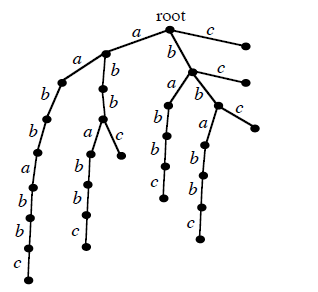
\includegraphics[width=0.45\linewidth]{graphics/suffix-trie-example.png}
\end{center}

Sprawdzenie, czy słowo $w$ jest podsłowem $t$ polega po prostu na sprawdzeniu, czy w drzewie sufiksowym $Trie(t)$ istnieje ścieżka zgodna z kolejnymi literami słowa $w$.

Pewnym ułatwieniem rozważań na drzewach sufiksowych jest zastosowanie specjalnego znaku $\$ \notin \A$ na końcu $t$. W ten sposób zapewniamy, że każdy sufiks $t$ kończy się w liściu tj. żaden sufiks nie jest prefiksem innego sufiksu.

\begin{problem}{}{}
  Dla dowolnego $n$ pokaż tekst $t$ długości $n$ taki, że rozmiar drzewa sufiksowego jest możliwie największy.
\end{problem}

% Słowo: a^n b^n a^n b^n c

Ponieważ podstawowe drzewo sufiksowe może mieć rozmiar większy niż liniowy, to wygodniejsze jest przejście na skompresowane drzewo sufiksowe (\emph{suffix tree}) $ST(t)$ tj. drzewo, w którym ściągnięto wszystkie wierzchołki stopnia $2$ różne od korzenia. Każda krawędź w drzewie zamiast odpowiadać pojedynczej literze, odpowiada teraz pewnemu słowu z $\A^+$. Dowolne dwie krawędzie wychodzące z tego samego wierzchołka odpowiadają słowom, których największych prefiks jest pusty (tj. różnią się pierwszym znakiem).
Oczywiście sprawdzenie, czy $w$ jest podsłowem $t$ przebiega dokładnie tak samo jak poprzednio.

\begin{theorem}{}{}
  Skompresowane drzewo sufiksowe dla dowolnego słowa $t$ o długości $n$ ma rozmiar $O(n)$.
\end{theorem}

\begin{proof}
  Wiemy, że drzewo $ST(t)$ ma co najwyżej $n$ liści (jeśli kończy się symbolem specjalnym, to ma dokładnie $n$). Z definicji każdy wierzchołek wewnętrzny drzewa skompresowanego ma co najmniej dwa poddrzewa, wobec tego liczba wierzchołków wewnętrznych musi być mniejsza od liczby liści.
\end{proof}

Z powyższych twierdzeń jasne jest, że konstrukcja skompresowanego drzewa sufiksowego przez najpierw zbudowanie, a następnie kompresję drzewa nieskompresowanego jest nieoptymalna.

% TODO s. 84-85 w crochermore1994text -- algorytmy naiwne

Optymalne podejścia przedstawione poniżej polegają na iteracyjnym rozbudowywaniu drzewa sufiksowego przez wstawianie kolejnych sufiksów we właściwej kolejności, od najdłuższego lub od najkrótszego. Okazuje się, że samo to jednak nie wystarczy:
\begin{problem}{}{}
  Dla dowolnego $n$ pokaż tekst $t$ ($|t| = n$) taki, że wstawianie sufiksów do drzewa sufiksowego w dowolnej kolejności zaczynając zawsze od korzenia wymaga $\Theta(n^2)$ operacji.
\end{problem}

\subsubsection{Algorytm McCreighta}

W omawianiu algorytmów będziemy korzystać oznaczenia $ST(t, i)$ jako (tymczasowego) drzewa słownikowego, zawierającego $i$ najdłuższych sufiksów $t$. Oznaczmy przez $leaf(i)$ liść wstawiony przy przejściu z $ST(t, i - 1)$ do $ST(t, i)$, odpowiadający sufiksowi $t[i..n]$. Dodatkowo, $head(i) = parent(leaf(i))$.

Ponadto, zdefiniujmy dla każdego wierzchołka $v$ funkcję $word(v)$ przypisującą mu słowo złożone z etykiet ścieżki od korzenia do $v$.
Jest to szczególnie użyteczne do definicji linków sufiksowych, wykorzystywanego w algorytmie: jeśli $word(v) = aw$ ($a \in \A$, $w \in \A^*$), to $S[v] = u$, gdzie $u$ jest wierzchołkiem, dla którego $word(u) = w$.

\begin{code}
\captionof{listing}{Algorytm McCreighta budowania drzewa sufiksowego}
\inputminted{python}{code/suffix-tree/mccreight.py}
\label{alg:mccreight-suffix-tree}
\end{code}

W dowodzie optymalności algorytmu McCreighta wykorzystywane będą następujące trzy własności:
\begin{problem}{crochemore1994text}{s. 91}
  Pokaż, że $head(i)$ jest potomkiem $S[head(i - 1)]$ w $ST(t, i)$.
\end{problem}

\begin{problem}{crochemore1994text}{s. 91}
  Pokaż, że $S[v]$ jest potomkiem $S[parent(v)]$ dla dowolnego $v$ w każdym $ST(t, i)$.
\end{problem}

\begin{problem}{}{}
  Pokaż, że $depth(v) \le depth(S[v]) + 1$ dla dowolnego $v \neq head(i)$ w każdym $ST(t, i)$.
\end{problem}

\begin{theorem}{}{}
  Algorytm McCreighta zwraca poprawne drzewo sufiksowe.
\end{theorem}

\begin{proof}
  Na początek załóżmy, że dla dowolnego $i = 2, 3, \ldots, n$ mamy zbudowane $ST(t, i - 1)$ oraz wszystkie wierzchołki wewnętrzne $ST(t, i - 1)$ inne niż $head(i - 1)$ mają dobrze zdefiniowane $S[v]$ (samo $S[head(i - 1)]$ też może być zdefiniowane wcześniej, ale nie musi). Ten niezmiennik jest utrzymany przez cały algorytm.

  Oczywiście $ST(t, 1)$ złożone z korzenia $r$, liścia $l_1$ i krawędzi między nimi z etykietą $t$ spełnia te warunki.
  
  Korzystając obu własności z problemów powyżej wiemy, że $S[parent(head(i - 1)]$ jest dobrze zdefiniowany oraz istnieje ścieżka z $S[parent(head(i - 1)]$ do $S[head(i - 1)]$ w $ST(t, i - 1)$ -- jedynie z tym zastrzeżeniem, że może kończyć się ,,w środku'' krawędzi tj. z $head(i - 1)$ jako wierzchołkiem skompresowanym.
  
  Wystarczy zatem dodać wierzchołek $leaf(i)$, być może rozbijając krawędź i tworząc nowy wierzchołek $head(i - 1)$, oraz nadać wartość $S[head(i - 1)]$ tak, żeby $S[head(i - 1)]$ było przodkiem $head(i)$, aby stworzyć drzewo, które jest $ST(t, i)$ oraz ma dobrze zdefiniowane $S[v]$ dla wszystkich wierzchołków wewnętrznych $v$ poza $head(i)$.
\end{proof}

\begin{theorem}{}{}
  Algorytm McCreighta ma złożoność $O(n \log{|\A|})$.
\end{theorem}

\begin{proof}
  Złożoność czasowa algorytmu wynika wprost z trzech faktów.
  
  Po pierwsze, poza funkcjami \texttt{fast\_find} i \texttt{slow\_find} algorytm wykonuje stałą liczbę operacji w każdej iteracji -- a zatem $O(n)$ operacji łącznie.
  Dla alfabetu $\A$ znalezienie w wierzchołku odpowiedniej krawędzi zaczynającej się od danego symbolu wynosi $O(\log{|\A|})$. Wszystkie pozostałe operacje wykonywane są w czasie stałym.

  Po drugie, niech funkcja \texttt{fast\_find} schodzi od wierzchołka $S[parent(head(i - 1))]$ w dół do wierzchołka $head(i)$ po dokładnie $d_i$ krawędziach. Wówczas wiemy, że
  \begin{align*}
    depth(head(i - 1)) \le depth(S[head(i - 1)]) + 1 = depth(head(i)) - d_i + 1.
  \end{align*}
  Wobec tego całkowita liczba przejść po krawędziach w funkcji \texttt{fast\_find} wynosi
  \begin{align*}
    \sum_{i = 2}^{n + 1} d_i \le \sum_{i = 2}^{n + 1} \left(depth(head(i)) - depth(head(i - 1)) + 1\right) \le depth(head(n)) + n \le 2 n
  \end{align*}

  Po trzecie, funkcja \texttt{slow\_find} w $i$-tej iteracji algorytmu wykonuje $s_i$ porównań, gdzie zachodzi $s_i \le |word(head(i))| - |word(head(i - 1))|$. Analogicznie jak powyżej, łączna liczba operacji jest ograniczona z góry przez $O(n)$.
\end{proof}

Warto zauważyć, że jeśli $S[head(i - 1)]$ jednak jest dobrze określone w $i$-tym kroku algorytmu, to możemy od razu przejść do tego wierzchołka, zamiast wykonywać przejście przez rodzica $head(i - 1)$ (tzw. \emph{up-link-down}). Taka optymalizacja nie zmienia jednak asymptotycznego czasu wykonania algorytmu.

\begin{problem}{crochemore1994text}{s. 93-94}
  Pokaż, że jeśli w Algorytmie \ref{alg:mccreight-suffix-tree} zamiast \texttt{fast\_find} użyjemy funkcji \texttt{slow\_find}, to dla dowolnego $n$ istnieje tekst $t$ długości $n$ taki, że konstrukcja $ST(t)$ wymaga czasu $\Omega(n^2)$.
\end{problem}

% Przykład: a^n

\subsubsection{Algorytm Ukkonena}

Algorytm Ukkonena polega na tym, że w tym przypadku budowane jest w zasadzie poprawne drzewo sufiksowe dla kolejnych prefiksów słowa $t$.
W trakcie wykonania algorytmu wyznaczamy dokładnie taką samą tablicę linków sufiksowych jak w algorytmie McCreighta.

\begin{code}
\captionof{listing}{Algorytm Ukkonena budowania drzewa sufiksowego}
\inputminted{python}{code/suffix-tree/ukkonen.py}
\label{alg:ukkonen-suffix-tree}
\end{code}

\begin{problem}{}{}
  Pokaż, że wartości $S[v]$ wyznaczane w algorytmach McCrieghta i Ukkonena są identyczne.
\end{problem}

\begin{theorem}{}{}
  Algorytm Ukkonena zwraca poprawne drzewo sufiksowe.
\end{theorem}

\begin{proof}
  Przede wszystkim zauważmy, że każdy nowododany liść pozostaje zawsze liściem do samego końca wykonania algorytmu -- w ten sposób $leaf(i)$ nie tylko reprezentuje sufiks $t[i]$ w $ST(t, i)$, ale również sufiks $t[i..j]$ w $ST(t, j)$ dla dowolnego $j \ge i$.
  
  Należy przy tym pamiętać, że w rzeczywistości, inaczej niż w powyższym algorytmie, pamiętamy nie całą etykietę na krawędzi, tylko parę liczb oznaczających początek i koniec etykiety w tekście. Wystarczy zatem ustawić indeksy końcowe w liściach na $+\infty$, unikając w ten sposób problemu z dodawaniem kolejnych znaków na końcach liści.
  
  Aby z $ST(t, i - 1)$ otrzymać $ST(t, i)$ wystarczy wstawić do drzewa wszystkie sufiksy słowa $t[1..i]$. Załóżmy jednak, że pewnym momencie natrafimy na (być może skompresowany) wierzchołek $v$, dla którego już istnieje (być może skompresowany) wierzchołek $v'$ spełniający $word(v) = word(v') \, t[i]$. Wówczas wiemy, że w drzewie nieskompresowanym dla wszystkich wierzchołków $u$ odpowiadających sufiksom słowa $word(v)$ istnieją wierzchołki $u'$ takie, że $word(u) = word(u') \, t[i]$. Wobec tego wszystkie mniejsze sufiksy słowa $t[1..i]$ już muszą istnieć.
  
  Idea algorytmu jest zatem taka: w $i$-tej iteracji wychodzimy od $head(i - 1)$ (zob. dowód algorytmu McCreighta) i chodząc po linkach sufiksowych rozbudowujemy drzewo o nowe liście zgodnie z $t[i]$ aż do momentu, gdy natrafimy na istniejący (może skompresowany) wierzchołek. Tak otrzymane drzewo (gdybyśmy zastąpili wszystkie indeksy końcowe $+\infty$ przez $i$) jest drzewem sufiksowym $ST(t, i)$.
\end{proof}

\begin{theorem}{}{}
  Algorytm Ukkonena ma złożoność $O(n \log{|\A|})$.
\end{theorem}

\begin{proof}
  Wszystkie operacje poza \texttt{fast\_find} wymagają czasu $O(\log{|\A|})$ na każdą iterację głównej pętli.
  
  Pętla \texttt{while} za każdym razem dodaje jeden liść, więc podczas całego wykonania algorytmu funkcja \texttt{fast\_find} zostanie wykonana $O(n)$ razy.
  Ponieważ wiemy, że $S[v]$ przyjmuje dokładnie takie same wartości, jak w algorytmie McCreighta, to również tu całkowita liczba odwiedzionych wierzchołków w funkcji \texttt{fast\_find} wyniesie $O(n)$.
\end{proof}

\subsubsection{Dalsze zagadnienia}

\citet{giegerich1997ukkonen} pokazali, że chociaż teoretyczne idee u podstaw wszystkich trzech algorytmów się różnią, to istnieje głębokie podobieństwo strukturalne. W szczególności można pokazać, że algorytmy McCreighta i Ukkonena wykonują dokładnie te same ciągi abstrakcyjnych operacji, a zatem możliwe jest tłumaczenie krok po kroku wykonania jednego algorytmu na drugi. Również algorytm Weinera przypomina strukturalnie algorytm Ukkonena z tą różnicą, że jest budowany ,,od końca'' i przez to korzysta jedynie z ,,przybliżonych'' linków.

Okazuje się, że możliwa jest konstrukcja drzewa sufiksowego w czasie $O(n)$, niezależnym od $\A$ \citep{farach1997optimal}. Wymaga to co prawda utożsamienia alfabetu z podzbiorem liczb naturalnych zamiast z dowolnym zbiorem z liniowym porządkiem, ale w przeciwieństwie do sortowania nie stanowi żadnego problemu.

Drzewa sufiksowe umożliwiają nie tylko szybkie obliczanie zapytań o przynależność, ale mogą również służyć do rozwiązywania kilku innych problemów.

\begin{problem}{crochemore2002jewels}{Theorem 5.2, s. 59-60}
  Pokaż, jak w czasie $O(m)$ odpowiadać na zapytania, ile razy słowo $w$ ($|w| = m$) występuje w tekście $t$, gdy mamy skonstruowane $ST(t)$.
\end{problem}

\begin{proof}
Mając zbudowane drzewo sufiksowe, idziemy od korzenia w dół czytając kolejne symbole $w$, a czasami posuwamy się po wewnętrznej etykiecie pewnej krawędzi. Wówczas zbiór wystąpień odpowiada zbiorowi liści w poddrzewie węzła, do którego udało nam się w ten sposób dojść. Liczbę takich liści możemy ustalić bardzo łatwo: budując drzewo sufiksowe możemy od razu obliczyć w każdym węźle trzymać ile liści jest w jego poddrzewie. Jeżeli po drodze nie dało się dalej schodzić po drzewie, oznacza to, że $w$ nie jest podsłowem słowa $t$, więc odpowiedzią jest zero.
\end{proof}

\begin{problem}{crochemore2002jewels}{Lemma 5.1, s. 63}
  Pokaż, jak w czasie $O(n)$ policzyć, ile różnych podsłów zawiera słowo $t$ ($|t| = n$).
\end{problem}

\begin{proof}
Gdybyśmy zbudowali takie pełne drzewo sufiksowe bez kompresji, to wówczas jest to po prostu drzewo trie wszystkich sufiksów danego słowa. Wówczas liczba różnych podsłów słowa $n$ jest po prostu równa liczbie wierzchołków w stworzonym drzewie. W przypadku, gdy budujemy drzewo sufiksowe z kompresją, aby nie mieć kwadratowego rozmiaru całej struktury, należy również policzyć wierzchołki w zbudowanym drzewie, ale dodatkowo licząc wierzchołki liczymy je z odpowiednimi wagami, które wynikają z tego, że wierzchołki w skompresowanym drzewie sufiksowym są tak naprawdę ścieżkami wierzchołków i je też należy uwzględnić, co możemy zrobić bardzo łatwo, poprzez popatrzenie jakie etykiety są trzymane w wierzchołkach i dodając odpowiednie krotności. Możemy to wszystko zrobić jednym przejściem po drzewie, skąd wynika liniowa złożoność względem długości słowa.
\end{proof}

\begin{problem}{crochemore2002jewels}{Theorem 5.3, s. 62}
  Pokaż, jak w czasie $O(n k)$ wyznaczyć najdłuższe wspólne podsłowo dla zbioru słów $\{t_i: 1 \le i \le k\}$ długości co najwyżej $n$.
\end{problem}

\begin{proof}
Rozwiązanie jest oczywiście bardzo proste. Wystarczy zbudować drzewo sufiksowe, ale nie dla każdego słowa osobno, ale jedno wspólne. Robimy to w ten sposób, że najpierw budujemy drzewo sufiksowe dla pierwszego słowa. Następnie wstawiamy do niego sufiksy drugiego słowa, trzeciego itd aż do $k$-tego, z tą różnicą, że wstawiając słowa, w wierzchołkach pamiętamy sobie informacje jaki sufiks tędy przechodzi w dół, tzn. każdy wierzchołek ma informacje na temat tego, sufiksy którego słowa przez niego przechodziły. Wówczas odpowiedzią, czyli najdłuższym wspólnym podsłowem, będzie najgłębiej położony węzeł w naszym drzewie zbudowanym dla $n$ słów, przez który przeszedł jakiś sufiks każdego słowa. Oczywiście można tego LCSa bardzo łatwo odtworzyć jak już mamy taki najgłębszy wierzchołek o tej własności. Wystarczy przejść się od korzenia do niego i zobaczyć jakie etykiety mijaliśmy po drodze.
\end{proof}

\subsubsection{Algorytm Weinera}

Algorytm Weinera, historycznie najwcześniejszy algorytm optymalny, polega na budowaniu drzewa sufiksowego od prawej do lewej. Zauważmy, że dzięki przeglądaniu tekstu w tej kolejności gwarantujemy, że w $i$-tym kroku budowana struktura danych jest pełnoprawnym drzewem sufiksowym dla słowa $t[(n - i - 1)..n]$.

Tak jak w algorytmie McCreighta, najważniejszą częścią algorytmu jest efektywne wyznaczanie linków między wierzchołkami drzewa -- z tą różnicą, że w tym przypadku są to linki odwrotne do linków sufiksowych.
Definiujemy je następująco: jeśli $word(v) = w$ ($w \in \A^*$) oraz $t[i] = a$, to $link_a[v] = u$, gdzie $u$ jest pewnym wierzchołkiem, dla którego $word(u) = a \, word(v)$.

Niniejsza implementacja jest oparta na uproszczonej wersji algorytmu, zamieszczonej w \citet{breslauer2013near}.
\begin{code}
\captionof{listing}{Algorytm Weinera budowania drzewa sufiksowego}
\inputminted{python}{code/suffix-tree/weiner.py}
\label{alg:suffix-tree-weiner}
\end{code}

\begin{problem}{}{}
  Pokaż, że Algorytm \ref{alg:suffix-tree-weiner} wylicza w każdej iteracji poprawne przejścia $link[v, c] = u$.
\end{problem}

\begin{problem}{}{}
  Pokaż, że Algorytm \ref{alg:suffix-tree-weiner} zwraca poprawne drzewo sufiksowe.
\end{problem}

\begin{problem}{}{}
  Pokaż, że Algorytm \ref{alg:suffix-tree-weiner} działa w czasie $O(n \log{|\A|})$.
\end{problem}

\subsection{Tablica sufiksowa}

Tablica sufiksowa jest dużo prostszą strukturą, wprowadzoną jako alternatywa dla drzew sufiksowych równolegle w \citep{gonnet1992new} i \citep{manber1993suffix}.
Wartości tablicy dla słowa $t$ długości $n$ definiujemy następująco:
\begin{align*}
    SA[i] = |\{j: t[j..n] \le t[i..n]\}|,
\end{align*}
czyli na $i$-tej pozycji mamy początkowy indeks $i$-tego najmniejszego sufiksu w porządku leksykograficznym.

Naiwny algorytm liczenia tablicy $SA$ wymaga czasu $O(n^2 \log{n})$, gdy wykorzystujemy sortowanie wymagające $O(n \log{n})$ porównań, ponieważ każde porównanie wymaga w najgorszym przypadku czasu $O(n)$.

Można również obliczyć tablicę $SA$ na podstawie zadanego drzewa sufiksowego w czasie $O(n)$: wystarczy przejrzeć drzewo wgłąb lub rekurencyjnie zgodnie z kolejnością liter w alfabecie. Zwróćmy uwagę, że Algorytm \ref{alg:suffix-array-from-suffix-tree} wyznacza długości słów na podstawie znajomości tekstu i aktualnej głębokości przeszukiwania.

\begin{code}
\captionof{listing}{Algorytm budowania tablicy sufiksowej na podstawie drzewa sufiksowego}
\inputminted{python}{code/suffix-array/from-suffix-tree.py}
\label{alg:suffix-array-from-suffix-tree}
\end{code}

\subsubsection{Algorytm Karpa-Millera-Rosenberga}

Algorytm \emph{prefix-doubling}, zaproponowany w \citep{karp1972rapid}, opiera się na pomyśle prostej rekurencji. Załóżmy, że dla podsłów $t[i:i + k]$\footnote{Ściślej chodzi nam o $t[i:\min \{i + k, n\}]$ -- albo można równoważnie założyć, że na końcu dodajemy nieskończony ciąg symboli $\$$.} dla pewnego $k \ge 1$ oraz $1 \le i \le n$ mamy dostęp do funkcji $rank(i, k)$, zwracającej numer $t[i:i + k]$ w porządku leksykograficznym.
Wówczas wystarczy umieć wyznaczać na jej podstawie efektywnie wartości $rank(i, 2k)$ dla wszystkich $1 \le i \le n$.

\begin{code}
\captionof{listing}{Algorytm Karpa-Millera-Rosenberga budowania tablicy sufiksowej}
\inputminted{python}{code/suffix-array/kmr.py}
\label{alg:suffix-array-kmr}
\end{code}

\begin{lemma}{crochemore2007algorithms}{Lemma 4.8, s. 169-170}
  Dla dowolnych $1 \le i \le n$ oraz $k \ge 1$ wartość $rank(i, 2k)$ jest równa pozycji pary $(rank(i, k), rank(i + k, k))$ w porządku leksykograficznym na wszystkich takich parach.
\end{lemma}

\begin{proof}
  Z założenia, $rank(i, k) < rank(j, k)$ wtedy i tylko wtedy, gdy $t[i: i + k] < t[j: j + k]$ oraz $rank(i, k) = rank(j, k)$ wtedy i tylko wtedy, gdy $t[i: i + k] = t[j: j + k]$ dla dowolnych $i$, $j$, $k$.

  Jeśli $t[i: i + k] < t[j: j + k]$, to oczywiście zachodzi $t[i: i + 2 k] < t[j: j + 2 k]$ dla dowolnych $i$, $j$, $k$.
  Podobnie jeśli $t[i: i + k] = t[j: j + k]$ oraz $t[i + k + 1: i + 2 k] = t[j + k + 1: j + 2 k]$, to również $t[i: i + 2 k]$ < $t[j: j + 2 k]$ dla dowolnych $i$, $j$, $k$.

  Składając te wszystkie obserwacje razem, otrzymujemy wprost, że $t[i: i + 2 k]$ < $t[j: j + 2 k]$ wtedy i tylko wtedy, gdy $rank(i, 2 k) < rank(j, 2 k)$ dla dowolnych $i$, $j$, $k$.

  Aby zakończyć dowód wystarczy zaobserwować, że dla dwóch sąsiednich elementów w porządku $rank(i, 2 k)$ nie może istnieć żaden element rozdzielający je w porządku $(rank(i, k), rank(i + k, k))$.
\end{proof}

\begin{corollary}{}{}
  Algorytm \ref{alg:suffix-array-kmr} zwraca poprawną tablicę sufiksową.
\end{corollary}

\begin{proof}
  Po $\log{n}$ iteracjach głównej pętli otrzymujemy z $rank(i, 1)$ tablicę wartości $rank(i, n)$ -- a to z definicji jest dokładnie tablica sufiksowa.
\end{proof}

\begin{theorem}{}{}
  Algorytm \ref{alg:suffix-array-kmr} wykonuje się w czasie $O(n \log{n})$.
\end{theorem}

\begin{proof}
  Całkowita złożoność algorytmu \ref{alg:suffix-array-kmr} zależy od zastosowanego sortowania.
  Jeśli jest to sortowanie pozycyjne (\emph{radix sort}), to pojedyncza iteracja wymaga czasu $O(n)$. Iteracji mamy dokładnie $\log{n}$.
\end{proof}

\subsubsection{Algorytm K\"arkk\"ainena-Sandersa}

Algorytm \emph{skew}, wprowadzony w \citep{karkkainen2003simple}, umożliwia zejście do liniowego czasu obliczania tablicy sufiksowej.
Wymaga on założenia o tym, że alfabet można utożsamić ze zbiorem liczb naturalnych. W przeciwieństwie jednak np. do problemu sortowania w algorytmach tekstowych jest to założenie bardzo naturalne i często spotykane w praktyce (podobnie jak założenie, że $|\A| = O(1)$).

Sednem algorytmu K\"arkk\"ainena-Sandersa jest zamiana słowa $t$ na słowo $t'$ takie, że $|t'| = \frac{2}{3} |t|$.
Zauważmy, że bez straty ogólności możemy założyć, że słowo $t$ jest długości podzielnej przez $3$ -- wystarczy dołożyć na koniec odpowiednią liczbę znaków $\# \notin \A$ takich, że $\# > a$ dla każdego $a \in \A$.

Dokładniej, niech $triple(i)$ oznacza pozycję $t[i:i+3]$ wśród wszystkich unikalnych trzyliterowych podsłów $t$ posortowanych leksykograficznie.
Tworzymy nowe słowo $t'$ w następujący sposób:
\begin{align*}
  t' = triple(1) \cdot triple(4) \ldots \cdot triple(2) \cdot triple(5) \ldots
\end{align*}
Zwrócony wynik dla tego słowa umożliwia odrębne posortowanie sufiksów $t$ osobno dla zbiorów
\begin{align*}
  P_{12} & = \left\{1 \le i \le n: i \mod 3 \in \{1, 2\}\right\} \\
  P_0 & = \left\{1 \le i \le n: i \mod 3 = 0\right\}.
\end{align*}
Co więcej, na podstawie danego $t'$ możliwe jest scalenie również częściowych tablic sufiksowych dla $P_{12}$ i $P_0$.

\begin{code}
\captionof{listing}{Algorytm K\"arkk\"ainena-Sandersa budowania tablicy sufiksowej}
\inputminted{python}{code/suffix-array/skew.py}
\label{alg:suffix-array-skew}
\end{code}

\begin{problem}{}{}
  Pokaż że \ref{alg:suffix-array-skew} na podstawie $t'$ wyznacza poprawnie tablicę sufiksów dla $P_{12}$.
\end{problem}

\begin{problem}{}{}
  Pokaż że \ref{alg:suffix-array-skew} na podstawie $t'$ wyznacza poprawnie tablicę sufiksów dla $P_0$.
\end{problem}

\begin{theorem}{}{}
  Algorytm \ref{alg:suffix-array-skew} na podstawie $t'$ poprawnie scala tablice sufiksów dla $P_{12}$ i $P_0$.
\end{theorem}

\begin{proof}
  Na mocy założenia mamy dostępne posortowane listy sufiksów osobno dla indeksów należących do $P_{12}$ i $P_0$.
  
  Scalenie odbywa się zgodnie z funkcją \emph{merge} identyczną jak w algorytmie mergesort. Mamy 2 przypadki:
  \begin{enumerate}
    \item jeśli mamy $i \in P_{12}$ takie, że $i \mod 3 = 2$ oraz pewne $j \in P_0$, to wiemy, że $i + 1, j + 1 \in P_{12}$ -- wystarczy zatem porównać ze sobą pary $(t[i], S[i + 1])$ i $(t[j], S[j + 1])$,
    \item jeśli mamy $i \in P_{12}$ takie, że $i \mod 3 = 1$ oraz pewne $j \in P_0$, to wiemy, że $i + 2, j + 2 \in P_{12}$ -- wówczas postępujemy podobnie, tylko porównujemy trójki $(t[i], t[i + 1], S[i + 2])$ i $(t[j], t[j + 1], S[j + 2])$.
  \end{enumerate}
  Zauważmy, że $S[i + 1]$, $S[i + 2]$ lub $t[i + 1]$ mogą nie istnieć (podobnie dla $j$). Wówczas wystarczy zwracać wartości, które będą zawsze mniejsze od wartości odpowiednio z $S$ lub $\A$.
\end{proof}

\begin{theorem}{}{}
  Czas działania algorytmu \ref{alg:suffix-array-skew} wynosi $O(n)$.
\end{theorem}

\subsubsection{Wykonywanie zapytań w czasie $O(m \log{n})$}

Sprawdzanie, czy słowo $w$ o długości $m$ występuje w tekście $t$ dla danej tablicy sufiksowej $SA(t)$ jest wykonalne w czasie $O(m \log{n})$: wystarczy zwykłe binarne wyszukiwanie słowa $w$ w $SA(t)$.

Co więcej, tablica sufiksowa umożliwia nie tylko zliczenie wszystkich wystąpień słowa $w$ w tekście w czasie $O(m \log{n})$, ale również odnalezienie ich w czasie $O(m \log{n} + k)$. Wystarczy tylko wyszukać pozycje odpowiadające słowom $w$ oraz $w\#$, gdzie $\# \notin \A$ oraz $a < \#$ dla każdego $a \in \A$. Pozycje te wyznaczają w tablicy $SA(t)$ sekwencję początków sufiksów, dla których $w$ musi być prefiksem -- chociaż niekoniecznie w kolejności rosnącej.

\subsubsection{Wykonywanie zapytań w czasie $O(m + \log{n})$}

\todo[inline]{Algorytm Manbera-Myersa}

\subsubsection{Dalsze zagadnienia}

\citet{li2018optimal} pokazali algorytm obliczania tablicy sufiksowej w czasie $O(n)$ wymagający zaledwie $O(1)$ dodatkowej pamięci.

\subsection{Tablica największych wspólnych prefiksów}

\todo[inline]{Konstrukcja tablicy LCP.}

\begin{theorem}{}{}
  Algorytm Kasai zwraca poprawną tablicę sufiksową.
\end{theorem}

\begin{proof}
  Weźmy dwa dowolne sufiksy słowa $t$ sąsiednie w porządku leksykograficznym tj. zaczynające się na pozycjach $SA[i]$ oraz $SA[i + 1]$ dla pewnego $1 \le i \le n - 1$. Niech długość najdłuższego wspólnego prefiksu $LCP(t[SA[i]:n], t[SA[i + 1]:n]) = k$ dla pewnego $k \ge 0$.

  Weźmy teraz $j$ takie, że $SA[j] = SA[i] + 1$, tj. $t[SA[j]:n] = t[SA[i] + 1:n]$. Wówczas wiemy, że
  \begin{align*}
    LCP(t[SA[j]:n], t[SA[j + 1]:n]) \ge \max\{LCP(t[SA[i]:n], t[SA[i + 1]:n]) - 1, 0\},
  \end{align*}
  ponieważ $t[SA[j]:n] < t[SA[j + 1]:n] \le t[SA[i + 1] + 1:n]$
  oraz
  \begin{align*}
    LCP(t[SA[j]:n], t[SA[i + 1] + 1:n])
        & = LCP(t[SA[i] + 1:n], t[SA[i + 1] + 1:n]) \\
        & = \max\{LCP(t[SA[i]:n], t[SA[i + 1]:n]) - 1, 0\}.
  \end{align*}
  Wykorzystujemy tu prosty fakt, że jeśli mamy dowolne słowa $w_1 \le w_2 \le w_3$, to $LCP(w_1, w_2) \ge LCP(w_1, w_3)$.

  Jeśli nie istnieje szukane $j$, to $SA[i] = n$, a zatem rzecz jasna $t[SA[i] + 1:n] = \varepsilon$, a zatem jego najdłuższy wspólny prefiks z dowolnym innym podsłowem wynosi $k = 0$.
\end{proof}

\begin{theorem}{}{}
  Liczba różnych podsłów dla słowa $t$ ($|t| = n$) wynosi
  \begin{equation*}
    \binom{n}{2} - \sum_{i = 1}^{n - 1} LCP[i]
  \end{equation*}
\end{theorem}

\begin{proof}
  Wystarczy policzyć podsłowa zaczynające się na pozycjach $SA[i + 1]$ dla $0 \le i \le n - 1$ tj. prefiksy $t[SA[i + 1]:n]$ niebędące prefiksami słów $t[SA[j]:n]$ dla $1 \le j \le i$.
  
  Ponieważ sufiksy są posortowane, to wiemy, że każdy prefiks $t[SA[i + 1]:n]$ długości $0 \le k < LCP[i]$ już wystąpił wcześniej -- w szczególności jako prefiks $t[SA[i]:n]$.
  
  Dalej, wiemy że $t[SA[i]:n] < t[SA[i + 1]:SA[i + 1] + LCP[i] + 1]$, ponieważ słowa są posortowane oraz $t[SA[i + 1] + LCP[i] + 1]$ jest z definicji $LCP$ pierwszym znakiem różnym w słowach $t[SA[i]:n]$ i $t[SA[i + 1]:n]$. Oczywiście z przechodniości relacji $<$ wynika, że również
  \begin{align*}
    t[SA[j]:n] \le t[SA[i]:n] < t[SA[i + 1]:SA[i + 1] + LCP[i] + k]
  \end{align*}
  dla wszystkich $k \ge 1$ oraz $1 \le j \le i$, a zatem każdy prefiks $t[SA[i + 1]:n]$ długości większej niż $LCP[i]$ na pewno nie jest prefiksem $t[SA[j]:n]$ dla $1 \le j \le i$.
  
  $t[SA[i + 1]:n]$ ma łącznie $n - SA[i + 1]$ prefiksów, więc takich prefiksów jest oczywiście $n - SA[i + 1] - LCP[i]$. Dla $i = 0$ oczywiście będzie to tylko $n - SA[1]$.
  Ostatecznie, całkowita liczba różnych słów wynosi
  \begin{align*}
    \sum_{i = 0}^{n - 1} \left(n - SA[i + 1]\right) - \sum_{i = 1}^{n - 1} LCP[i - 1] = \binom{n}{2} - \sum_{i = 1}^{n - 1} LCP[i],
  \end{align*}
  ponieważ $\sum_{i = 0}^{n - 1} \left(n - SA[i + 1]\right)$ to zarazem liczba wszystkich (niekoniecznie różnych) podsłów w tekście.
\end{proof}

\subsection{Suffix trays}

\todo[inline]{Uzupełnić -- ale z niskim priorytetem}

\section{Największy sufiks}

\begin{algorithm}[H]
    \caption{Największy leksykograficznie sufiks}
    \Input{Słowo $w \in \A^+$ ($|w| = m$)}
    \Output{Liczba $1 \le i \le m$ taka, że $w[i..m]$ jest największym leksykograficznie sufiksem $w$.}
\end{algorithm}

\subsection{Algorytm na bazie tablicy prefikso-sufiksów}

\begin{lemma}{}{}
  Jeśli dla dowolnego słowa $w$ słowo $u$ jest maksymalnym sufiksem $w[1..(j - 1)]$ a słowo $v$ jest takim sufiksem słowa $w[1..(j - 1)]$, że $u w[j] < v w[j]$, to $v$ jest prefikso-sufiksem $u$.
\end{lemma}

\begin{proof}
  Skoro $u$ jest maksymalnym sufiksem $w[1..(j - 1)]$, to $u > v$. Jeśli $v$ nie było prefiksem $u$, to istniałaby pozycja $1 \le i \le |v|$ taka, że $v[i] < u[i]$. Ale wówczas $uy \ge u > vy$ dla dowolnego $y \in \A^*$ -- sprzeczność z tym, że $u w[j] < v w[j]$.
\end{proof}

\begin{lemma}{}{}
  Jeśli dla dowolnego słowa $w$ słowo $u$ jest maksymalnym sufiksem $w[1..(j - 1)]$ oraz dla pewnego prefikso-sufiksu $v$ słowa $u$ zachodzi $u w[j] < v w[j]$, to dla wszystkich słów $v'$ takich, że $v'$ jest prefikso-sufiksem $u$ i $v$ jest prefikso-sufiksem $v'$ zachodzi $u w[j] < v' w[j] < v w[j]$.
\end{lemma}

\begin{proof}
  Dla dowolnego $v'$ będącego prefikso-sufiksem $u$ istnieje słowo $x$ takie, że $u = v' x$.
  Ponieważ $u$ jest maksymalnym sufiksem $w[1..(j - 1)]$, to $u = v' x > v x$, ponieważ $v x$ też jest sufiksem $w[1..(j - 1)]$.
  Wówczas zachodzi $v x < u < u w[j] < v w[j]$, a zatem $x < w[j]$.
  Wobec tego $u w[j] = v' x w[j] < v' w[j]$.
  
  Wiemy, że $v w[j] > u w[j]$. Skoro $|u| > |v|$, to $v w[j] > u[1..(|v| + 1)] y$ dla dowolnego $y \in \A^*$.
  Łatwo sprawdzić, że każde $v'$ takie, że $v'$ jest prefikso-sufiksem $u$ i $v$ jest prefikso-sufiksem $v$ jest postaci $u[1..(|v| + 1)] y$.
\end{proof}

\begin{corollary}{}{}
  Jeśli dla dowolnego słowa $w$ słowo $u$ jest maksymalnym sufiksem $w[1..(j - 1)]$ a słowo $v w[j]$ jest maksymalnym sufiksem słowa $w[1..j]$, to wystarczy schodzić po prefikso-sufiksach $u$ dopóki to możliwe.
\end{corollary}

\begin{code}
\captionof{listing}{Wyszukiwanie największego leksykograficznie sufiksu}
\inputminted{python}{code/maximum-suffix/from-prefix-suffix.py}
\label{alg:maximum-suffix-from-prefix-suffix}
\end{code}

\begin{problem}{}{}
  Pokaż, że $B[j]$ to taka liczba, że $w[1..B[j]]$ jest największym prefikso-sufiksem maksymalnego sufiksu $w[1..j]$.
\end{problem}

\subsection{Algorytm o stałej pamięci}

\begin{code}
\captionof{listing}{Wyszukiwanie największego leksykograficznie sufiksu w pamięci $O(1)$}
\inputminted{python}{code/maximum-suffix/constant-space.py}
\label{alg:maximum-suffix-constant-space}
\end{code}

\begin{problem}{}{}
  Pokaż, że algorytm \ref{alg:maximum-suffix-constant-space} wyznacza poprawnie największy leksykograficznie sufiks.
\end{problem}

\section{Odległość edycyjna}

\begin{algorithm}[H]
    \caption{Odległość edycyjna}
    \Input{Słowa $t_1, t_2 \in \A^+$ ($|t_i| = n_i$ dla $i = 1, 2$)}
    \Output{Minimalna liczba operacji typu \emph{insert}, \emph{delete} i \emph{substitute} przeprowadzająca słowo $t_1$ w $t_2$.}
\end{algorithm}

Zwróćmy uwagę, że analogiczny problem, w którym dozwolona jest tylko operacja \emph{substitute} to obliczanie odległości Hamminga. Można ją wprost wyznaczyć przeglądając $t_1$ i $t_2$ od lewej do prawej, zliczając pozycje, dla których $t_1[i] \neq t_2[i]$.

Podstawowy algorytm obliczania odległości edycyjnej sprowadza się do sekwencyjnego obliczania wartości funkcji rekurencyjnej
\begin{align*}
  d_e(i, j) =
  \begin{cases}
    0 & \text{gdy $i = 0$ lub $j = 0$,} \\
    d_e(i - 1, j - 1) & \text{gdy $t_1[i] = t_2[j]$,} \\
    \min\{d_e(i - 1, j - 1), d_e(i - 1, j), d_e(i - 1, j - 1)\} + 1 & \text{gdy $t_1[i] \neq t_2[j]$.}
  \end{cases}
\end{align*}
Poprawność algorytmu wynika z indukcji ze względu na porządek par $(i, j)$. Czas działania algorytmu to $O(n_1 n_2)$.
Jak widać z powyższego wzoru, do obliczeń wystarczy zapamiętanie poprzedniego wiersza lub kolumny, więc wymagana pamięć wynosi $O(\min\{n_1, n_2\})$.

\begin{code}
\captionof{listing}{Obliczanie odległości edycyjnej w czasie $O(n_1 n_2)$ i pamięci $O(\min\{n_1, n_2\})$}
\inputminted{python}{code/other/edit-distance.py}
\label{alg:edit-distance}
\end{code}

Technika może być łatwo uogólniona do dowolnych macierzy ocen, przypisujących różne wagi za odległości dla operacji \emph{insert}, \emph{delete} i \emph{substitute}. Przykładem takiego wykorzystania są rodziny macierzy PAM i BLOSUM dla algorytmów dopasowań ciągów w zastosowaniach bioinformatycznych.

Można również łatwo zamienić problem na obliczanie funkcji podobieństwa jako maksymalnej (zamiast minimalnej) wartości dla danej macierzy operacji, tym razem interpretowanej jako macierz nagród \citep{sellers1974theory}.

\subsection{Technika czterech Rosjan}

Dla obliczeń macierzowych istnieje ogólna technika przyspieszania obliczeń, nazywana \emph{Four Russians speedup}\footnote{Najbardziej znanym z autorów był Jefim Dinic, znany również z algorytmu dla znajdowania maksymalnego przepływu w grafach.}.

Główna idea tej metody polega na podziale wejścia na małe bloki o niewielkim zakresie wartości.
Załóżmy, że pewien problem jest w ogólności rozwiązywany przez funkcję $y_n = f(y_{n - 1}, x_n)$, a jedna iteracja wymaga czasu $F(n)$ -- więc całość wykonuje się w czasie $\sum_{i = 1}^{n - 1} F(i)$.

Załóżmy teraz, że każda pozycja wejściowa pochodzi z małego zbioru $X$, a każda pozycja wyjściowa również z małego zbioru $Y$.
Wówczas dla dowolnego $k$ zawsze możemy obliczyć z wyprzedzeniem tablicę wszystkich $|X|^k |Y|$ wartości funkcji $f^{(k)}$, czyli $k$-krotnego złożenia $f$.
Wówczas można policzyć $f_n$ wykorzystując $\frac{n}{k}$ wyszukiwania w tablicy. Całkowity czas działania (zakładając stały dostęp do tablicy wartości) wynosi zatem
\begin{align*}
  |X|^k |Y| \sum_{i = 1}^{k - 1} F(i) + \frac{n}{k}.
\end{align*}
Przykładowo dla $F(n) = n^2$, $|X| = O(1)$ i $|Y| = O(n)$ wystarczy dobrać $k = \log_{|X|}{n}$, aby zmniejszyć czas wykonania z $O(n^3)$ do $O(n^2 \log^3{n})$.

Metoda ta używana jest m.in. do mnożenia i odwracania macierzy binarnych, a także do efektywnego liczenia domknięcia przechodniego grafu. Można ją również wykorzystać do optymalizacji algorytmu obliczającego odległość edycyjną \citep{masek1980faster}. Technika ta również uogólnia się na różnorodne macierze nagród i kar.

\todo[inline]{Algorytm i dowód}
% Gusfield 302-307
% w czasie $O\left(nm \frac{1}{\log{m}}\right)$

\section{Najdłuższy wspólny podciąg}

\begin{algorithm}[H]
    \caption{Najdłuższy wspólny podciąg}
    \Input{Zbiór słów $T = \{t_1, t_2, ..., t_k\} \subseteq \A^+$ takich, że $|t_i| \le n$ dla $1 \le i \le k$.}
    \Output{Słowo $t$ będące najdłuższym podciągiem wszystkich słów z $T$.}
\end{algorithm}

Problem najdłuższego wspólnego podciągu jest powiązany z problemem odległości edycyjnej.
Dla $|T| = 2$ niech $d(t_1, t_2)$ oznacza odległość dla dopuszczalnych operacji \emph{insert} i \emph{delete}.
Wówczas zachodzi
\begin{align*}
    |t_1| + |t_2| = 2 |t| + d(t_1, t_2),
\end{align*}
wystarczy bowiem zauważyć, że $t_1$ w $t$ przeprowadzają wszystkie operacje \emph{delete} a $t$ w $t_2$ -- \emph{insert}.

\subsection{Algorytm Needlemana-Wunscha}

Podstawowy algorytm obliczania najdłuższego wspólnego podciągu dla dwóch słów jest prostym rozszerzeniem algorytmu \ref{alg:edit-distance}. Jedyna różnica polega na konieczności trzymania całej tablicy odległości.
Odtwarzanie wyniku następuje na podstawie przejścia po ścieżce od ostatniej wartości tj. $d(t_1, t_2)$ do początku, odpowiadającemu $d(\epsilon, \epsilon)$.
Wybieramy rzecz jasna tylko te przejścia, które spełniają relację $\min$ w równaniu rekurencyjnym.

Oczywiście można odtwarzać kolejne przejścia i uzgodnione litery na podstawie $t_1$, $t_2$ porównując odpowiednie wartości macierzy $d$ -- lub też można zapisywać odpowiednie informacje równolegle w trakcie wypełniania tablicy $d$.

\begin{code}
\captionof{listing}{Obliczanie najdłuższego wspólnego podsłowa w czasie i pamięci $O(n_1 n_2)$}
\inputminted{python}{code/approximate-string-matching/needleman-wunsch.py}
\label{alg:lcs-needleman-wunsch}
\end{code}

\subsection{Algorytm Hirschberga}

Ponieważ dla dostatecznie dużych $n_1$ i $n_2$ w praktyce pamięć jest bardziej dotkliwą barierą niż czas, można zastanowić się nad usprawnieniem algorytmu, aby wykorzystywał tylko $O(\min\{n_1, n_2\})$ pamięci.

Okazuje się, że wystarczy zastosować podejście dziel-i-rządź. Z jednej strony jasne jest, że odpowiadająca najdłuższemu podciągowi optymalna ścieżka od punktu $(0, 0)$ do $(n_1, n_2)$ w macierzy $d$ musi przejść przez pewien punkt $(i, j)$ dla dowolnego $0 \le i \le n_1$. Możemy zatem wybrać $i$ w połowie aktualnie rozpatrywanego przedziału.

Znalezienie $j$ nie jest trudne. Okazuje się, że wystarczy do tego obserwacja z poniższego lematu:
\begin{problem}{}{}
  Punkt $(i, j)$ leży na (pewnej) optymalnej ścieżce w macierzy $d$ wtedy i tylko wtedy, gdy
  \begin{align*}
      j = \arg\max \{0 \le k \le n_2: d(t_1[1..i], t_2[1..k]) + d(\bar{t_1[i..n_2]}, \bar{t_2[k..n_2]})\}.
  \end{align*}
\end{problem}

\begin{code}
\captionof{listing}{Obliczanie najdłuższego wspólnego podsłowa w czasie $O(n_1 n_2)$ i pamięci $O(\min\{n_1, n_2\})$}
\inputminted{python}{code/approximate-string-matching/hirschberg.py}
\label{alg:lcs-hirschberg}
\end{code}

\subsection{Inne wyniki}

W ramach wyników negatywnych dla problemu odległości edycyjnej wiadomo, że nie istnieje żaden algorytm dla obliczania odległości edycyjnej o złożoności $\Theta(n^{2 - \varepsilon})$ dla dowolnego $\varepsilon > 0$, o ile Strong Exponential Time Hypothesis jest prawdziwa \citep{backurs2015edit}. Twierdzenie to zachodzi nawet dla przypadku alfabetu binarnego \citep{bringmann2015quadratic}.

\section{Dopasowanie wzorca z wieloznacznikami}

Wprowadźmy teraz symbol specjalny $?$ jako wieloznacznik lokalny (\emph{don't care symbol}), pasujący do każdego pojedynczego symbolu z $\A$.

\begin{definition}{}{}
  Relacja $\simeq$ jest relacją {\bf\textit{dopasowania z wieloznacznikiem lokalnym}} tj. $u \simeq v$ wtedy i tylko wtedy, gdy $|u| = |v|$ oraz dla wszystkich $1 \le i \le |u|$ zachodzi $u[i] = v[i]$ lub $u[i] =\,?$, lub też $v[i] =\,?$.
\end{definition}

\begin{algorithm}[H]
    \caption{Wyszukiwanie wszystkich wystąpień wzorca z wieloznacznikami lokalnymi w tekście}
    \Input{Słowa $t, w \in (\A \cup \{?\})^+$ ($|t| = n$, $|w| = m$)}
    \Output{Zbiór liczb $S = \{1 \le i \le n: t[i..(i + m - 1)] \simeq w\}$.}
\end{algorithm}

Istnieje bardzo pomysłowy algorytm obliczania wszystkich wystąpień wzorca z wieloznacznikami lokalnymi w tekście, oparty o szybką transformatę Fouriera.
Jak wiadomo, FFT umożliwia obliczanie dla dwóch wektorów $X$ i $Y$ o długości odpowiednio $n$ i $m$ (zakładając, że $n \ge m$) w czasie $O(n \log{n})$ operacji splotu tj. takiego $Z$, że dla wszystkich $0 \le i \le n - m$ zachodzi
\begin{align*}
  Z[i] = \sum_{j = 0}^{m - 1} X[i + j] Y[m - 1 - j].
\end{align*}
Zwróćmy uwagę, że -- wyjątkowo -- mamy w tym przypadku indeksowanie od $0$.

\begin{code}
\captionof{listing}{Obliczanie wszystkie wystąpień wzorca z wieloznacznikami lokalnymi w tekście}
\inputminted{python}{code/approximate-string-matching/basic-fft.py}
\label{alg:string-matching-dont-care-basic-fft}
\end{code}

\begin{theorem}{}{}
  Algorytm \ref{alg:string-matching-dont-care-basic-fft} wyznacza poprawnie wszystkie wystąpień wzorca z wieloznacznikami lokalnymi w tekście.
\end{theorem}

\begin{proof}
Kluczowa obserwacja jest następująca: wybierzmy dwie różne litery $a, b \in \A$ i wyznaczmy odpowiednio dla wszystkich $0 \le i \le n - 1$ oraz $0 \le j \le m - 1$
\begin{align*}
    X[i] = \text{$1$ gdy $t[i + 1] = a$}, & \text{w przeciwnym przypadku $X[i] = 0$,} \\
    Y[j] = \text{$1$ gdy $w[m - j] = b$}, & \text{w przeciwnym przypadku $Y[j] = 0$.}
\end{align*}
Wówczas
\begin{align*}
    Z[i] = \sum_{j = 0}^{m - 1} X[i + j] Y[m - 1 - j] = |\{0 \le j \le m - 1: t[i + j + 1] = a \land w[j + 1] = b \}|,
\end{align*}
a zatem $Z[i]$ jest po prostu zliczeniem wszystkich niedopasowań między tekstem $t[i + 1..i + m]$ a wzorcem $w$,
takich że w tekście występuje $a$, a we wzorcu $b$.
Powtarzając to dla wszystkich par liter w alfabecie możemy zliczyć wszystkie niedopasowania między $t[i + 1..i + m]$ a $w$ -- a zatem dopasowania będą na na tych pozycjach, na których niedopasowań brak.
\end{proof}

Jak łatwo zauważyć, algorytm \ref{alg:string-matching-dont-care-basic-fft} działa w czasie $O(n \log{n} |\A|^2)$.

%\section{Przybliżone dopasowanie wzorca}


\section{Najkrótsze wspólne nadsłowo}

\begin{algorithm}[H]
    \caption{Najkrótsze wspólne nadsłowo}
    \Input{Zbiór słów $T = \{t_1, t_2, \ldots, t_k\} \subseteq \A^+$ takich, że $|t_i| \le n$ dla $1 \le i \le k$.}
    \Output{Słowo $t$ będące najkrótszym nadsłowem wszystkich słów z $T$.}
\end{algorithm}

Bez straty ogólności zakładamy, że dla żadnej pary słów $t_i$ i $t_j$ nie zachodzi sytuacja, że $t_i$ jest podsłowem $t_j$. Gdyby taka sytuacja wystąpiła, to moglibyśmy usunąć $t_i$ z $T$ bez zmiany optymalnego rozwiązania.

W ogólności problem jest trudny, zarówno dla krótkich słów, jak i dla małych alfabetów.
\begin{theorem}{gallant1980finding}{}
  Niech $T = \{t_1, t_2, ..., t_k\}$ i $|t_i| = 3$ dla $1 \le i \le k$.
  Problem znalezienia najkrótszego nadsłowa dla $T$ jest NP-trudny.
\end{theorem}

\begin{theorem}{gallant1980finding}{}
  Niech $T = \{t_1, t_2, ..., t_k\}$ oraz $|\A| = 2$.
  Problem znalezienia najkrótszego nadsłowa dla $T$ jest NP-trudny.
\end{theorem}

Pokazano, że problem znalezienia najkrótszego nadsłowa należy do klasy złożoności MAX-SNP, a zatem istnieje stała $c > 1$, dla której nie istnieje algorytm $c$-przybliżony dla tego problemu. \citet{vassilevska2005explicit} dowiodła, że $c \ge \frac{1217}{1216}$, \citet{karpinski2013improved} poprawili to do $c \ge \frac{333}{332}$.

\begin{problem}{apostolico-galil}{Theorem 8.2, s. 239-240}
  Niech $T = \{t_1, t_2, ..., t_k\}$ przy $|t_i| \le 2$ dla $1 \le i \le k$.
  Pokaż, jak możliwe jest wyznaczenie najkrótszego nadsłowa $t$ dla $T$ w czasie wielomianowym.
\end{problem}

\subsection{Algorytm zachłanny}

\todo[inline]{Kod i dowód złożoności}

Niech $T = \{c(ab)^k, (ba)^k, (ab)^kc\}$, wówczas algorytm zachłanny najpierw złoży ze sobą dwa skrajne ciągi, a zatem $t_{APX} = (ba)^kc(ab)^kc$, $|t_{APX}| = 4 k + 2$, podczas gdy $t_{OPT} = c(ab)^{k + 1}c$, $|t_{OPT}| = 2 k + 4$.

Została postawiona hipoteza, że algorytm zachłanny jest $2$-przybliżony, ale dotychczas udało się tylko pokazać współczynnik aproksymacji równy $4$ \citep{blum1994linear}, a następnie poprawić współczynnik go do $3.5$ \citep{kaplan2005approximation}.

Zamiast porównywać długości słowa optymalnego i zwróconego przez algorytm możemy też zmienić kryterium optymalizacji.
Naturalnym alternatywnym kryterium wydaje się wielkość kompresji:

\begin{algorithm}[H]
    \caption{Wspólne nadsłowo o największej kompresji}
    \Input{Zbiór słów $T = \{t_1, t_2, \ldots, t_k\} \subseteq \A^+$ takich, że $|t_i| \le n$ dla $1 \le i \le k$.}
    \Output{Słowo $t$ będące nadsłowem wszystkich słów z $T$ i maksymalizujące $d = \sum_{i = 1}^k |t_i| - |t|$.}
\end{algorithm}
Oczywiście zbiór rozwiązań optymalnych dla obu problemów jest identyczny.

Okazuje się, że przy tych założeniach można pokazać, że algorytm zachłanny jest $2$-przybliżony tj. osiąga kompresję taką, że $2 d_{APX} \ge d_{OPT}$ \citep{tarhio1988greedy}.

\subsection{Inne wyniki}

Oprócz algorytmu zachłannego opracowywano inne algorytmy o współczynnikach aproksymacji kolejno $\frac{8}{3}$ \citep{armen19962}, $\frac{5}{2}$ \citep{kaplan2005approximation, sweedyk2000boldmath}, $\frac{57}{23}$ \citep{mucha2013lyndon} i -- obecnie najlepszego -- $\frac{71}{30}$ \citep{paluch2014better}.
Większość z tych rezultatów polega na odpowiednio sprytnej redukcji do odpowiednio efektywnego algorytmu dla problemu maksymalnej ścieżki komiwojażera w grafie asymetrycznym.

Dodatkowo, jeśli przyjmiemy, że $|t_i| = r \ge 3$, to istnieje algorytm $\frac{r^2 + r - 4}{4r - 6}$-przybliżony \citep{golovnev2013approximating}. W \citet{braquelaire2018improving} ten wynik został nieznacznie poprawiony -- pozostaje on nadal jednak lepszy niż algorytm ogólny tylko dla $2 \le r \le 7$.


\nocite{*}
\printbibliography

\end{document}
